\documentclass[11pt]{article}

\usepackage{amsmath}
\numberwithin{equation}{section}
\usepackage{subfigure}
\usepackage{amssymb}
\usepackage{amsthm}
\usepackage{blindtext}
\usepackage[parfill]{parskip}
\usepackage{graphicx}
\usepackage{textcomp}
\usepackage[utf8]{inputenc}
\usepackage{float}
\usepackage{diagbox}
\usepackage{tikz}
\usepackage{pgfgantt}
\usepackage{nicefrac}
\usepackage{caption}
\usepackage{setspace}
\usepackage{geometry}
\usepackage[toc,page]{appendix}
\usepackage{lipsum}
\usepackage[export]{adjustbox}
\usepackage[T1]{fontenc}
\usepackage{textcomp}
\usepackage{epsfig,graphics}
\usepackage{titlesec}
\usepackage{multirow}

\newcommand{\projectTitle}{Matrix Solvers for Stochastic Galerkin Schemes}
\newcommand{\fullname}{Alexander Harvey}
\newcommand{\degreeTitle}{MSc Advanced Computer Science}
\newcommand{\session}{2017/18}

 \geometry{
 a4paper,
 total={210mm,297mm},
 left=25mm,
 right=25mm,
 top=25mm,
 bottom=20mm,
 }

\newcommand{\frontcover}{
% The title page:
\begin{titlepage}
\newgeometry{left=25mm,right=25mm,top=45mm,bottom=0.1cm}

\begin{minipage}[t]{7cm}
\noindent\textbf{\Large{School of Computing}}\\
{\fontfamily{ptm}\selectfont 
\uppercase{faculty of engineering}
}
\end{minipage}
\hfill
\begin{minipage}[t]{7cm}
\vspace*{-25pt}

\includegraphics[scale=0.2,right]{logo_black.png}
\vspace*{-1pt}
\end{minipage}

\noindent\makebox[\linewidth]{\rule{\paperwidth}{0.4pt}}

\centering
\vspace*{37mm}
\textbf{\Large\projectTitle}\\
\vspace*{10mm}
\textbf{\large\fullname}\\
\vspace*{10mm}
\textbf{Submitted in accordance with the requirements for the degree of}\\
\textbf{\degreeTitle}\\
\vspace*{10mm}
\session\\
\restoregeometry
\end{titlepage}
}

\newcommand{\subsubsubsection}[1]{\paragraph{#1}\mbox{}\\}
\setcounter{secnumdepth}{4}
\setcounter{tocdepth}{4}

\onehalfspacing

\begin{document}

\frontcover

\newpage

\textbf{Summary}


\newpage

\textbf{Acknowledgements}
I would sincerely like to thank my project supervisor, Thomas Ranner, for his invaluable guidance and support during this project. His encouragement and feedback throughout has made it a thoroughly rewarding experience. I would also like to thank the University of Leeds and the School of Computing, as well as all the lecturers who have taught me throughout this year, as I have thoroughly enjoyed studying my MSc.

\newpage

\pagenumbering{roman}

\tableofcontents

\clearpage

\pagenumbering{arabic}

\section{Introduction}
This project involves exploring methods for solving matrix equations that arise from partial differential equations (PDEs) and investigates how a problem's structure can be exploited when dealing with equations in this form. Exploiting a problem based on its structure is not often possible when using conventional methods to solve PDEs, which usually involve stacking the unknowns of a problem into a single vector. By formulating a problem as a matrix equation and taking advantage of its structure, dramatic improvements in efficiency can be made compared to the conventional approach. The project then goes on to investigate how the methods explored can be applied to random PDEs (PDEs with uncertain input). Uncertainty can arise in PDEs for various different reasons (unknown coefficients, initial conditions or boundary conditions) in a variety of applications (physics \cite{Swanson}, \cite{Pryhara}, \cite{Breit}, \cite{Holm}, biology \cite{Bressloff}, \cite{Edwards}, finance \cite{Shreve03}, \cite{Shreve04}). Random PDEs are much harder to solve as opposed to regular PDEs as the solution has an element of `randomness' to it; it is not simply deterministic. 

Firstly, a model problem will be derived using Poisson's equation and different methods for solving this problem will be explored and compared. We will then proceed to introduce elements of uncertainty to the problem to see the effect this has and explore methods that can be used to solve this problem. We begin by constructing the matrix form of Poission's equation.

\subsection{Possion Equation}
As an example, we define the spatial domain $\mathcal{D} = \{(x,y) : 0 \leq x \leq 1, \; 0 \leq y \leq 1 \}$ and let $u: \mathcal{D} \to \mathbb{R}$ be the solution of Poisson's equation:
	\begin{alignat}{1} 
	-u_{xx} - u_{yy} = {} & f \quad \text{ on } \mathcal{D} \nonumber \\
	u = {} & 0 \quad \text{ on } \partial \mathcal{D}
	\end{alignat}
as shown in Figure \ref{fig:domain1}.

\begin{figure}[H]
\begin{tikzpicture}
\draw (0,0) rectangle (6,6);
\node at (3,3) {$-u_{xx}-u_{yy}=f$};
\node at (-0.25,3) {$0$};
\node at (6.25,3) {$0$};
\node at (3,-0.25) {$0$};
\node at (3,6.25) {$0$};

\node at (-0.25,-0.25) {$(0,0)$};
\node at (-0.25,6.25) {$(0,1)$};
\node at (6.25,-0.25) {$(1,0)$};
\node at (6.25,6.25) {$(1,1)$};

\draw[->] (7,0) -- (8,0);
\draw[->] (7,0) -- (7,1);
\node at (7.5,-0.25) {$x$};
\node at (6.75,0.5) {$y$};
\end{tikzpicture}
\centering
\caption{Domain for $-u_{xx}-u_{yy}=f$.}
\label{fig:domain1}
\end{figure}

The domain of this PDE can be discretised into a mesh with uniform spacing $h$ using the centred finite difference approximations:
	\begin{equation} 
	u_{xx} \approx \frac{u_{i-1j} - 2u_{ij} + u_{i+1j}}{h^2}
	\end{equation}
	\begin{equation}
	u_{yy} \approx \frac{u_{ij-1} - 2u_{ij} + u_{ij+1}}{h^2}
	\end{equation}
where $u_{ij} = u(x_i, y_j)$. The mesh is shown in Figure \ref{fig:domain2}.

\begin{figure}[H]
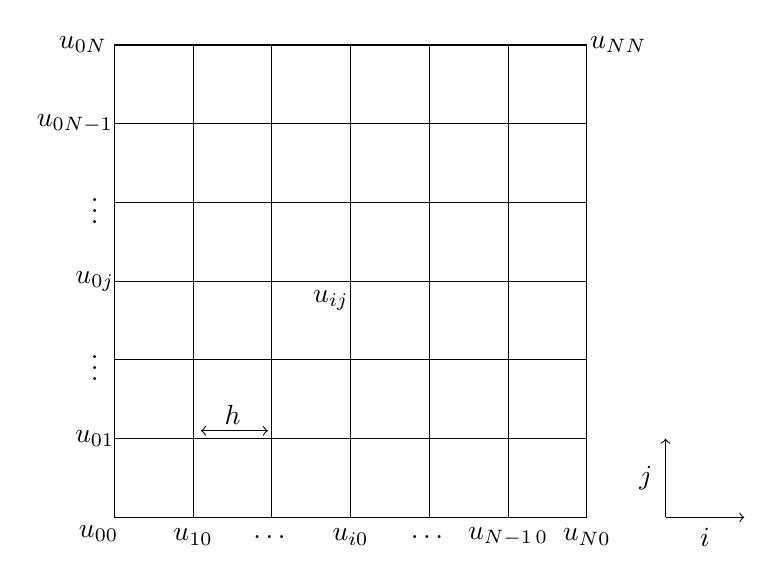
\begin{tikzpicture}
\draw (0,0) grid (6,6);
\node at (-0.2,-0.2) {$u_{00}$};
\node at (1,-0.25) {$u_{10}$};
\node at (2,-0.25) {$\dots$};
\node at (3,-0.25) {$u_{i0}$};
\node at (4,-0.25) {$\dots$};
\node at (5,-0.25) {$u_{N-1\,0}$};
\node at (6,-0.25) {$u_{N0}$};

\node at (-0.25,1) {$u_{01}$};
\node at (-0.25,2) {$\vdots$};
\node at (-0.25,3) {$u_{0j}$};
\node at (-0.25,4) {$\vdots$};
\node at (-0.5,5) {$u_{0N-1}$};
\node at (-0.4,6) {$u_{0N}$};

\node at (2.75,2.75) {$u_{ij}$};
\node at (6.4,6) {$u_{NN}$};

\draw[->] (7,0) -- (8,0);
\draw[->] (7,0) -- (7,1);
\node at (7.5,-0.25) {$i$};
\node at (6.75,0.5) {$j$};

\draw[<->] (1.1,1.1) -- (1.95,1.1);
\node at (1.5,1.3) {$h$};

\end{tikzpicture}
\centering
\caption{Discretised domain for $-u_{xx}-u_{yy}=f$.}
\label{fig:domain2}
\end{figure}

The discretised form of this PDE can then be solved by computing the equation:
	\begin{equation}
	f_{ij} = -\frac{1}{h^2} \big( u_{i-1j} - 2u_{ij} + u_{i+1j} \big) - \frac{1}{h^2} \big( u_{ij-1} - 2u_{ij} + u_{ij+1} \big)
	\end{equation}
at each internal grid point, meaning the system has $n^2$ unknowns with $n=N-2$. The traditional approach to solving this discretised form would be to write (1.4) as:
	\begin{equation}
	f_{ij} = -\frac{1}{h^2} \big( u_{i-1j} + u_{ij-1} - 4u_{ij} + u_{i+1j} + u_{ij+1}  \big)
	\end{equation}
and then stack all unknowns $u_{ij}$ into a single vector $u$, resulting in the linear system $Au=f$. We instead explore an alternative formulation.

\subsection{Sylvester Equation}
A Sylvester equation is a matrix equation of the form $AX + XB = C$, where $A$ is a $n \times n$ matrix, $B$ is a $m \times m$ matrix, and $X$ and $C$ are $n \times m$ matrices. We can write (1.4) as a Sylvester equation in the form:
	\begin{equation}
	TU + UT = F
	\end{equation}
where $T$, $U$ and $F$ are of size $n \times n$.

Let $\text{tridiag}(\beta,\alpha,\gamma)$ be defined as a tridiagonal matrix with $\alpha$ on the main diagonal and $\beta$ and $\gamma$ on the left and right diagonals, respectively. Then for (1.6) we have $T=-\frac{1}{h^2} \, \text{tridiag}(1,-2,1)$ and $U_{ij} = u(x_i, y_j)$, where $(x_i, y_j)$ are interior grid nodes for $i,j=1,\dots,n$. The system has $n$ unknowns in each direction meaning there is a total of $n^2$ unknowns. The matrix equation is visualised below:
\begin{eqnarray}
\frac{-1}{h^2} 
\begin{pmatrix}
-2 & 1 & 0 & \dots & 0 & 0 \\
1 & -2 & 1 & \dots & 0 & 0 \\
0 & 1 & -2 & \dots & 0 & 0 \\
\vdots & \vdots & \vdots & \ddots & \vdots & \vdots \\
0 & 0 & 0 & \dots & -2 & 1 \\
0 & 0 & 0 & \dots & 1 & -2 \\
\end{pmatrix}
\begin{pmatrix}
u_{11} & u_{12} & \dots & u_{1j} & \dots & u_{1n} \\
u_{21} & u_{22} & \dots & u_{2j} & \dots & u_{2n} \\
\vdots & \vdots & \ddots & \vdots & \dots & \vdots \\
u_{i1} & u_{i2} & \dots & u_{ij} & \dots & u_{in} \\
\vdots & \vdots & \vdots & \vdots & \ddots & \vdots \\
u_{n1} & u_{n2} & \dots & u_{nj} & \dots & u_{nn}
\end{pmatrix} \nonumber \\ \nonumber
+
\begin{pmatrix}
u_{11} & u_{12} & \dots & u_{1j} & \dots & u_{1n} \\
u_{21} & u_{22} & \dots & u_{2j} & \dots & u_{2n} \\
\vdots & \vdots & \ddots & \vdots & \dots & \vdots \\
u_{i1} & u_{i2} & \dots & u_{ij} & \dots & u_{in} \\
\vdots & \vdots & \vdots & \vdots & \ddots & \vdots \\
u_{n1} & u_{n2} & \dots & u_{nj} & \dots & u_{nn}
\end{pmatrix}
\frac{-1}{h^2} 
\begin{pmatrix}
-2 & 1 & 0 & \dots & 0 & 0 \\
1 & -2 & 1 & \dots & 0 & 0 \\
0 & 1 & -2 & \dots & 0 & 0 \\
\vdots & \vdots & \vdots & \ddots & \vdots & \vdots \\
0 & 0 & 0 & \dots & -2 & 1 \\
0 & 0 & 0 & \dots & 1 & -2 \\
\end{pmatrix}
= F
\end{eqnarray}
A variety of methods can now be used to solve this equation. These methods will be explored in Section 3. 

\subsection{Organisation}
The organisation of this report is as follows: Section 2 sets out the objectives and planning of the project, Section 3 explores different methods for solving a specific Sylvester equation, Section 4 introduces uncertainty into the problem studied in Section 3 and explores ways of solving this problem by building upon the knowledge gained in the previous section and finally, Section 5 is an evaluation of the project's success.

\newpage

\section{Scope and Schedule}
\subsection{Aim}
The first aim of this project is to study, implement and compare a range of matrix equation solvers. Following this, the project will look at ways of solving random PDEs and how the methods implemented can be applied to PDEs of this type.

\subsection{Objectives}
The objectives of this project are as follows:
\begin{itemize}
\item To carry out an extensive literature review on methods for solving matrix equations (both direct and iterative) from a variety of different sources, and to decide which of these methods are appropriate to implement by gaining a solid understanding of how they work.
\item To study ways of solving random PDEs and adapt methods that have already been considered in the project so that they can be used to solve PDEs of this type. 
\item To use and expand upon my programming experience to implement the chosen methods for solving matrix equations and random PDEs. 
\item To evaluate the implementation in each section by comparing and contrasting the methods implemented to decide which is the best suited for solving the given problem.
\item To clearly present the work carried out during the project by using and building upon my report writing skills.
\end{itemize}

\subsection{Deliverables}
The deliverables of this project include:
\begin{itemize}
\item The final report containing the details of the methods that have been studied, how they were implemented, an analysis and comparison of these methods, and then finally an evaluation of the success of the project.  
\item Code that successfully implements what has been studied in the project.
\end{itemize}

\subsection{Methodology}
The methodology of this project will involve studying academic publishings to gain an understanding of various methods for solving matrix equations and ways of solving random PDEs. Python will be the programming language of choice for the implementation because of my familiarity with it, the extensive amount of documentation available for it and the excellent libraries it has available. GitHub will be used for version control and the final report will be written using \LaTeX. 

%\subsection{Tasks, Milestones and Timeline}
%The steps of this project will be divided into iterations, with the problem in each iteration becoming successively more complex and difficult to solve. This is because understanding is a key part of this project, and so each iteration will build on the understanding of the last. Each iteration will consist of studying and applying matrix methods to the problem, implementing them in Python to solve the problem, evaluating the results and write up. Also rough deadlines will be given for when each iteration should be completed by, to ensure the project is on track at any given stage.
%
%The iterations are as follows:
%\begin{itemize}
%\item Introductory problem: $-u_{xx} - u_{yy} = 2 \pi^2 \sin{(\pi x)} \sin{(\pi y)}$ - deadline June 1st
%\item Problem introducing uncertainty: $-\varepsilon u_{xx} - \varepsilon u_{yy} = 2 \pi^2 \sin{(\pi x)} \sin{(\pi y)}$ - deadline June 22nd
%\item A Poisson equation on a surface defined by a height map (not yet derived) - deadline July 13th
%\item Application reaction-diffusion equation (not yet derived) - deadline August 3rd
%\end{itemize}
%
%If the project deadlines are met the remaining time will be dedicated to project evaluation, write up and any possible project extensions.

\newpage

\section{Matrix Solvers}
This section explores different methods for solving a particular matrix equation in Sylvester form. Sylvester equations appear in many applications, for example they frequently appear in signal processing \cite{Scottedward} and control theory \cite{Castelan}. We begin by forming a specific model problem. 

For spatial domain $\mathcal{D} = \{(x,y) : 0 \leq x \leq 1, \; 0 \leq y \leq 1 \}$ and $u: \mathcal{D} \rightarrow \mathbb{R}$, let $u(x,y) = \sin{(\pi x)} \sin{(\pi y)}$ be the exact solution of the equation:
\begin{alignat}{2}
-u_{xx} -u_{yy} = {} & f \quad & \text{ on } \mathcal{D} \nonumber \\
u = {} & 0 \quad & \text{ on } \partial \mathcal{D}
\end{alignat}
This gives:
\begin{equation}
\begin{split}
u_{xx} = u_{yy} = - \pi^2 \sin{(\pi x)} \sin{(\pi y)} \\
\implies f = 2 \pi^2 \sin{(\pi x)} \sin {(\pi y)}
\end{split}
\end{equation} 
The equation to be be solved is therefore:
\begin{alignat}{1}
-u_{xx} -u_{yy} = {} & 2 \pi^2 \sin{(\pi x)} \sin {(\pi y)} \quad \text{ on } \mathcal{D} \nonumber \\
u = {} & 0 \quad \text{ on } \partial \mathcal{D}
\end{alignat}
Using the centred finite difference approximations with uniform grid spacing $h$ to discretise the domain of this system, we have:
	\begin{equation}
	-\frac{1}{h^2} \big( u_{i-1j} - 2u_{ij} + u_{i+1j} \big) - \frac{1}{h^2} \big( u_{ij-1} - 2u_{ij} + u_{ij+1} \big) = F
	\end{equation}
with $F_{ij} = 2\pi^2 \sin(\pi x_i) \sin(\pi y_j)$, to be solved at each grid point for $i, j = 1, \dots n$, where $n$ is the total number of unknowns in each direction. The matrix form of this equation is therefore:
\begin{equation}
	TU + UT = F
\end{equation}
where $T=-\frac{1}{h^2} \, \text{tridiag}(1,-2,1)$, $U_{ij} = u(x_i, y_j)$ and $F_{ij} = 2 \pi^2 \sin(\pi x_i) \sin(\pi y_j)$ are all matrices of size $n \times n$ and $(x_i, y_j)$ are interior grid nodes for $i,j=1,\dots,n$. This form allows us to explore different methods for solving this equation and compare them to the exact solution $u = \sin(\pi x) \sin(\pi y)$. A plot of the exact solution, with $n=1000$, is given in Figure \ref{fig:solution}. 
\begin{figure}[H]
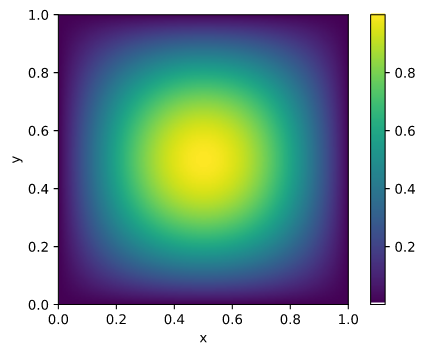
\includegraphics[scale=.5]{img/solution2.png}
\centering
\caption{Plot of the solution with $n=1000$.}
\label{fig:solution}
\end{figure} 

Throughout the following section, each of the implemented methods will be given a maximum execution time of 6000 seconds to compute a solution. If a method does not compute a solution in this time for a certain problem size, this will be specified in the results. If a method does not compute a solution because it needs more memory than is available, this will also be specified. All tests in this section (and throughout the report) will be run on a DEC-10 computer with 32GB of RAM and 8 cores. 

The following measurements will be given to evaluate the performance of each of the methods implemented:
\begin{itemize}
\item $n$: The number of unknowns in each direction for the system - the total number of unknowns is $n^2$. The mesh size will be continually refined by a factor of $\frac{1}{2}$, meaning the total number of unknowns in each direction will be doubled at each level, until either the time limit is reached or too much memory is used. The starting value will be $n=125$, which will allow for a range of problem sizes to be tested without running more tests than necessary.
\item Time(s): The time taken in seconds for the method to compute a solution to the problem. As previously stated the maximum time allowed will be 6000 seconds.
\item $|| u - u_h ||_{L^\infty} $: An error measurement which measures the maximum difference between the actual solution and computed solution for each $u$. Defined as:
 \[ || u - u_h ||_{L^\infty} = \text{max}_{ij} | u(x_i, y_i) - u_{ij} | \]
\item $|| u - u_h ||_{L^2} $: An error measurement which measures the average difference between the actual solution and computed solution for all $u$, defined as:
\[ || u - u_h ||_{L^2} = \sqrt{h^2 \sum | u(x_i,y_j) - u_{ij} |^2} \]
\item Experimental order of convergence (eoc): Measures the rate of convergence of a method as the problem size is increased \cite{Grau}. As we are using the centred finite difference approximations which are second order, this should be approximately 2.  Defined as:
\[ \text{eoc}(i) = \frac{\log(\nicefrac{E_i}{E_{i-1}})}{\log(\nicefrac{h_i}{h_{i-1}})} \]
where $E_i$ is the error (chosen here as $|| u - u_h ||_{L^\infty}$) and $h_i$ is the mesh size at level $i$. 
\item Experimental order of growth (eog): Measures the order of growth of the execution time of an algorithm as the problem size is increased (that is, the approximate time complexity). Defined as:
\[ \text{eog}(i) = \frac{\log(\nicefrac{t_{i}}{t_{i-1}})}{\log(\nicefrac{n_{i}}{n_{i-1}})} \]
where $t_i$ is the total execution time and $n_i$ is the problem size at level $i$.
\item No. iters (iterative methods only): The number of iterations taken for the method to converge to the given convergence tolerance.
\end{itemize}
All non-integer measurements will be given to five significant figures. It is worth noting that as the total number of unknowns, and therefore the problem size, is $n^2$, the best time complexity that an optimal solver can achieve is $O(n^2)$, as it must compute a solution for each unknown. Also, as each of the methods is solving the same equation, the differences in error for each of the methods should be small.

\subsection{Direct Methods}

\subsubsection{Kronecker Product}
A simple approach to solving this equation is to use the Kronecker product to rewrite (3.5) as a standard vector linear system \cite{Laub}. The Sylvester equation $AX + XB = C$ can be written as the standard vector linear system:
\begin{equation}
\mathcal{A}x = c
\end{equation}
with $\mathcal{A} = I \otimes A + B^* \otimes I$, where $I$ is the identity matrix, $B^*$ denotes the conjugate transpose of $B$, $x = \text{vec}(X)$\footnote{The vec operator reshapes a matrix into a vector by stacking the columns one after another.}, $c = \text{vec}(C)$ and $\otimes$ denotes the Kronecker product.

The equivalent linear system for the matrix equation $TU + UT = F$ is:
\begin{equation}
\mathcal{T}u = f
\end{equation}
where $\mathcal{T} = I \otimes T + T \otimes I$, $u = \text{vec}(U)$ and $f = \text{vec}(F)$.

This is the exact linear system that would be obtained from equation (1.5), that is, stacking all unknowns $u_{ij}$ into a single vector in the first place. Since the matrix $\mathcal{T}$ is sparse, this equation can be solved using a standard direct sparse solver. This approach provides a good base case for comparison. \texttt{sparse.linalg.spsolve} is a direct sparse solver from the SciPy library that uses a LU decomposition to solve a linear system. Using a LU decomposition to solve a linear system of size $n$ has time complexity, at most, $O(n^3)$. However, as we have used the Kronecker product to form our linear system, it has size $n^2$. We can therefore expect this method to run in worse than $O(n^3)$ (and no more than $O(n^6)$).

Results solving the equation using the Kronecker product to from a linear system and solving the system using \texttt{sparse.linalg.spsolve} are shown in Table \ref{table:kron direct}. As can be seen from the results, both of the errors decrease as the problem size $n$ is increased and the eoc is close to 2 for all $n$. This demonstrates that this method is solving the problem more and more accurately as the problem size is increased. As we increase $n$ the eog grows beyond $3$, which shows that this algorithm has worse than cubic time complexity for large $n$, as expected. For $n=4000$, this method results in a memory error. This is because \texttt{spsolve} tries to compute a (incomplete) LU decomposition of $\mathcal{T}$ which destroys the sparsity of the matrix and therefore requires much more memory to store it. The SciPy documentation notes that ``this solver assumes the resulting matrix X is sparse...If the resulting X is dense...consider converting A to a dense matrix and using \texttt{scipy.linalg.solve} or its variants.'' \texttt{scipy.linalg.solve} was tested to see how it would compare to the sparse solver. It was much slower for the problem sizes it was able to solve and resulted in a memory error for $n=500$.

\begin{table}[H]
\centering
\begin{tabular}{|c|c|c|c|c|c|}
\hline
$n$ & Time(s) & $|| u - u_h ||_{L^{\infty}}$ &$|| u - u_h ||_{L^{2}}$ & eoc & eog \\
\hline
125 & 0.18141 & $5.1807 \times 10^{-5}$ & $2.5904 \times 10^{-5}$ & - & - \\
250 & 0.60371 & $1.3054 \times 10^{-5}$ & $6.5275 \times 10^{-6}$ & 2.0001 & 1.7346 \\
500 & 4.1663 & $3.2767 \times 10^{-6}$ & $1.6384 \times 10^{-6}$ & 1.9999 & 2.7868 \\
1000 & 36.113 & $8.2082 \times 10^{-7}$ & $4.1041 \times 10^{-7}$ & 2.0000 & 3.1157 \\
2000 & 404.48 & $2.0539 \times 10^{-7}$ & $1.0267 \times 10^{-7}$ & 2.0001 & 3.4855 \\
\cline{2-6}
4000 & \multicolumn{5}{c|}{Memory Error} \\
\hline
\end{tabular}
\captionsetup{justification=centering}
\caption{Results obtained from solving the linear system $\mathcal{A} x = c$ using the direct solver  \texttt{sparse.linalg.spsolve} from the SciPy library.}
\label{table:kron direct}
\end{table}

\subsubsection{Bartels-Stewart Algorithm}
The Bartels-Stewart algorithm \cite{Bartels} can be used to solve the Sylvester equation $AX + XB = C$. 
This algorithm works by computing the Schur decompositions of the coefficient matrices $A$ and $B$, which are used to transform the equation into an equivalent form that has coefficient matrices that are upper and lower triangular. This triangular system can then be solved one element at a time and its solution is then used to obtain the solution to the original equation.

In the general case the algorithm is as follows:
\begin{enumerate}
\item Compute the Schur forms $A^* = PRP^*$ and $B=QSQ^*$.
\item Solve $R^*Y + YS = \hat{C}$ for $Y$, where $\hat{C} = P^*CQ$.
\item Compute $X=PYQ^*$.
\end{enumerate}
Here the matrices $R$ and $S$ are upper/lower triangular matrices with the eigenvalues of $A$ and $B$ on the diagonal, respectively. The matrices $P$ and $Q$ are unitary matrices whose columns are orthonormal sets of eigenvectors obtained from the eigenvectors of $A$ and $B$, respectively.

By breaking this algorithm down into its component parts, we can examine each part to see which is the most costly. The first step of the algorithm can be computed using \texttt{linalg.schur} from the SciPy library, which uses the QR algorithm and has time complexity $O(n^3)$ \cite{Parlett}. For the second step, each entry of $Y$ can be computed as:
\begin{equation}
Y_{ij} = \hat{C}_{ij} - \sum_{p=1}^{i-1} R_{ip}Y_{pj} - \sum_{q=1}^{j-1} Y_{iq}S_{qj}
\end{equation}
for $i,j=1, \dots, n$. This also has time complexity $O(n^3)$, as it will have a \texttt{for} loop running from $i=1$ to $n$, a nested \texttt{for} loop running from $j=1$ to $n$ and then two nested \texttt{for} loops which run from $p=1$ and $q=1$ to $i-1$ and $j-1$, respectively. The last step of the algorithm is a simple matrix multiplication, which has time complexity of at most $O(n^3)$. Therefore we can expect this algorithm to run in roughly $O(n^3)$. 

The algorithm simplifies for $TU+UT=F$. In this case the algorithm is as follows:
\begin{enumerate}
\item Compute the Schur form $T=PRP^*$.
\item Solve $R^*V + VR = \hat{F}$ for $V$, where $\hat{F} =  P^*FP$.
\item Compute $U=PVP^*$.
\end{enumerate}
As the matrix $T$ is symmetric, its eigenvectors are orthogonal \cite{Quandt}, implying that $R$ is now a diagonal matrix, which has the eigenvalues of $T$ on the diagonal. We can see this is true by examining the steps of the Schur decomposition. For a general matrix $A$, a Schur decomposition $A=PRP^*$ has 4 steps:
\begin{enumerate}
\item Find the eigenvalues of $A$.
\item Find the corresponding eigenvectors of $A$.
\item Compute an orthonormal set of eigenvectors using the eigenvectors of $A$, for example by using Gram-Schmidt orthogonalisation.
\item The eigenvectors found in Step 3 make up the columns of $P$. $R$ can now be found as $R=P^*AP$. 
\end{enumerate}
As the eigenvectors of $T$ are already orthogonal, they only need to be normalised in the 3rd step of the decomposition. This means that $R$ will be a diagonal matrix with the eigenvalues of $T$ on the diagonal.

This property reduces the complexity of the second step to $O(n^2)$, as only the diagonal elements need to be calculated making the two summations unnecessary. We can therefore expect the algorithm to run faster than in the general case and to be dominated by the first step. Consequently, we should now expect this algorithm to have, in the worst case, time complexity $O(n^3)$.

\subsubsection*{SciPy Solver}
The SciPy library has a built-in solver for solving Sylvester equations, \texttt{linalg.solve\_sylvester}, which uses the Bartels-Stewart algorithm. We can use this to test the general algorithm. Results using this solver are given in Table \ref{table:bartels scipy}. We can see from these results that this solver is much faster than using the Kronecker product and \texttt{spsolve}. The errors here are almost exactly the same as the errors in Table \ref{table:kron direct}, and up to $n=4000$, the eoc is very close to 2, but for $n=8000$ it moves beyond 2. The eog seems to change depending on the problem size, however, for large $n$ this method has close to cubic time complexity. Although it is difficult to analyse the steps of this solver directly, \texttt{solve\_sylvester} makes use of LAPACK, an optimised software library for solving linear algebra problems, to compute the Schur decomposition in the first step. LAPACK uses a couple of different methods for computing the eigenpairs of symmetric tridiagonal matrices \cite{Demmel}. It is likely that the method changes depending on the problem size, which causes the changes in the eog and the spike in the eoc for $n=8000$. 

\begin{table}[H]
\centering
\begin{tabular}{|c|c|c|c|c|c|}
\hline
$n$ & Time(s) & $|| u - u_h ||_{L^{\infty}}$ &$|| u - u_h ||_{L^{2}}$ & eoc & eog \\
\hline
125 & 0.059959 & $5.1807 \times 10^{-5}$ & $2.5904 \times 10^{-5}$ & - & - \\
250 & 0.11421 & $1.3054 \times 10^{-5}$ & $6.5275 \times 10^{-6}$ & 2.0001 & 0.92964 \\
500 & 1.9383 & $3.2767 \times 10^{-6}$ & $1.6384 \times 10^{-6}$ & 1.9999 & 4.0850  \\
1000 & 4.0920 & $8.2084 \times 10^{-7}$ & $4.1042 \times 10^{-7}$ & 2.0000 & 1.0780 \\
2000 & 32.029 & $2.0503 \times 10^{-7}$ & $1.0259 \times 10^{-7}$ & 2.0027 & 2.9685  \\
4000 & 279.95 & $4.9949 \times 10^{-8}$ & $2.4876 \times 10^{-8}$ & 2.0377 & 3.1277  \\
8000 & 2812.2 & $8.6380 \times 10^{-9}$ & $4.1216 \times 10^{-9}$ & 2.5321 & 3.3285 \\
\cline{2-6}
16000 & \multicolumn{5}{c|}{Time Limit Reached} \\
\hline
\end{tabular}
\caption{Results using SciPy's \texttt{linalg.solve\_sylvester}.}
\label{table:bartels scipy}
\end{table}

\subsubsection*{Simplified Implementation}

Results using the simplified version of this algorithm are shown in Table \ref{table:bartels simplified}. These results demonstrate that this simplified implementation is much faster than the SciPy solver. The errors up until $n=2000$ are very similar to the errors in the previous methods, and the eoc is again very close to 2 up until $n=4000$. After this point, the eoc starts decreasing rapidly and when $n=16000$ the error becomes bigger than when $n=8000$. These can be explained by the fact that \texttt{linalg.schur} is used to compute the Schur decomposition in the first step. \texttt{linalg.schur} uses the QR algorithm to approximate the eigenpairs of $T$ (as there is no general formula for calculating the eigenpairs of an arbitrary matrix of size $n>4$). From these results we can see that this approximation has a significant impact on the error for large $n$. The eog here demonstrates that this algorithm has better than cubic time complexity.
\begin{table}[H]
\centering
\begin{tabular}{|c|c|c|c|c|c|}
\hline
$n$ & Time(s) & $|| u - u_h ||_{L^{\infty}}$ &$|| u - u_h ||_{L^{2}}$ & eoc & eog \\
\hline
125 & 0.036654 & $5.1807 \times 10^{-5}$ & $2.5904 \times 10^{-5}$ & - & - \\
250 & 0.084191 & $1.3054 \times 10^{-5}$ & $6.5275 \times 10^{-6}$ & 2.0001 & 1.1997 \\
500 & 0.35179 & $3.2766 \times 10^{-6}$ & $1.6383 \times 10^{-6}$ & 2.0000 & 2.0630 \\
1000 & 1.2846 & $8.2081 \times 10^{-7}$ & $4.1041 \times 10^{-7}$ & 2.0000 & 1.8685 \\
2000 & 7.3734 & $2.0531 \times 10^{-7}$ & $1.0265 \times 10^{-7}$ & 2.0007 & 2.5210 \\
4000 & 40.664 & $4.8578 \times 10^{-8}$ & $2.4421 \times 10^{-8}$ & 2.0802 & 2.4634 \\
8000 & 291.47 & $1.5975 \times 10^{-8}$ & $7.9337 \times 10^{-9}$ & 1.6048 & 2.8415 \\
16000 & 1797.2 & $1.6116 \times 10^{-7}$ & $9.0649 \times 10^{-8}$ & -3.3349 & 2.6243 \\
\cline{2-6}
32000 & \multicolumn{5}{c|}{Memory Error} \\
\hline
\end{tabular}
\caption{Results using the simplified Bartels-Stewart algorithm.}
\label{table:bartels simplified}
\end{table}

Timing results of each step of the algorithm are given in Table \ref{table:bartels simplified steps}, where the headings of the table correspond to each step of the algorithm. These results show that this algorithm is largely dominated by computing the Schur decompositions in the first step, as expected.

\begin{table}[H]
\centering
\begin{tabular}{|c|c|c|c|c|c|}
\hline
$n$ & 1 & 2 & 3 & Total & eog \\
\hline
125 & 0.023111 & 0.013408 & 0.00013494 & 0.036654 & - \\
250 & 0.035753 & 0.047841 & 0.00059700 & 0.084191 & 1.1997 \\
500 & 0.15627 & 0.19206 & 0.0034585 & 0.35179 & 2.0630 \\ 
1000 & 0.49460 & 0.76522 & 0.024728 & 1.2846 & 1.8685 \\
2000 & 3.1751 & 4.0314 & 0.16686 & 7.3734 & 2.5210 \\
4000 & 25.373 & 14.011 & 1.2787 & 40.664 & 2.4634 \\
8000 & 218.92 & 61.979 & 10.566 & 291.47 & 2.8415 \\
16000 & 1433.7 & 277.08 & 86.375 & 1797.2 & 2.6243 \\
\hline
\end{tabular}
\caption{Timings for each step using the simplified Bartels-Stewart algorithm.}
\label{table:bartels simplified steps}
\end{table}

\subsubsection{Similarity Transformation}
A similarity transformation \cite{Simoncini} can be used to solve the Sylvester equation $AX + XB = C$. Assuming that the coefficient matrices $A$ and $B$ can be diagonalised, this method uses an eigendecomposition to reform the equation so that the solution can be easily obtained. The method is as follows:
\begin{enumerate}
\item Compute the eigendecompositions $P^{-1}AP = \text{diag}(\lambda_1, \dots, \lambda_n)$ and $Q^{-1}BQ = \text{diag}(\mu_1, \dots, \mu_m)$:
	\begin{enumerate}
	\item Compute the eigenpairs of $A$ and $B$
	\item Compute the inverses of $P$ and $Q$
	\end{enumerate}
\item Compute the solution $X = P \widetilde{X} Q^{-1}$, where $\widetilde{X}_{ij} = \frac{\widetilde{C}_{ij}}{\lambda_i + \mu_j}$ and $\widetilde{C} = P^{-1}CQ$.
\end{enumerate}
Here $\lambda_1, \dots, \lambda_n$ are the eigenvalues of $A$, $\mu_1, \dots, \mu_m$ are the eigenvalues of $B$ and the columns of $P$ and $Q$ are the eigenvectors of $A$ and $B$, respectively. We can analyse the steps of this algorithm as done previously to obtain the time complexity. Step 1a consists of computing the eigenpairs of $A$ and $B$, which in general is $O(n^3)$ \cite{Pan}. Step 1b computes the inverse of $P$ and $Q$ which is no more than $O(n^3)$. The last step involves matrix multiplication, which is at most $O(n^3)$. Therefore we can expect this algorithm in the general case to have, in the worst case, complexity $O(n^3)$, with the first step dominating.

For $TU+UT=F$ this method also simplifies. The steps are: 
\begin{enumerate}
\item Compute the eigendecomposition $P^{-1}TP = \text{diag}(\lambda_1, \dots, \lambda_n)$
	\begin{enumerate}
	\item Compute the eigenpairs of $T$
	\item Compute the inverse of $P$
	\end{enumerate}
\item Compute the solution $U = P \widetilde{U} P^{-1}$, where $\widetilde{U}_{ij} = \frac{\widetilde{F}_{ij}}{\lambda_i + \lambda_j}$ and $\widetilde{F}=P^{-1}FP$
\end{enumerate}
As before $\lambda_1, \dots, \lambda_n$ are the eigenvalues of $T$ and the columns of $P$ are the eigenvectors of $T$. The complexity of the first step can be drastically reduced. Using a result from \cite{Elliott}, we can compute the eigenvalues and eigenvectors directly as:
\begin{equation} 
\lambda_i = \frac{2}{h^2} \Big( 1 - \cos \Big( \frac{i \pi}{n+1} \Big) \Big) 
\end{equation}
and:
\begin{equation}
P_{ij} = \sqrt{\frac{2}{n+1}} \sin \Big( \frac{ij \pi}{n+1}  \Big) 
\end{equation}
which reduces the time complexity to $O(n)$, as $T$ has $n$ eigenpairs which all need to be computed and stored. Also, in this case the matrix $P$ is unitary, which means that $P^{-1} = P^T$ and so calculating the inverse of $P$ reduces to $O(n^2)$. This should result in a significant speed up compared to the general version of this algorithm.

An interesting fact to note here is that in this specific case the Schur decomposition and eigendecomposition of $T$ actually produce the same matrices. 

\subsubsection*{Numpy's \texttt{linalg.eig} function}
In the general case of this method, the eigenpairs can be computed using NumPy's \texttt{linalg.eig} function. The results of doing this are given in Table \ref{table:sim trans numpy}. Here we can see the errors for $n<8000$ are similar to that of the previous methods and the eoc is close enough to 2 to conclude that this method is solving the problem more and more accurately as the mesh size is decreased, up to $n=4000$. Similarly to the implementation of the Bartels-Stewart algorithm, for $n\geq 8000$ and the error grows when $n=16000$ and the eoc decreases significantly. As before, this is because \texttt{linalg.eig} is approximating the eigenpairs and this has a significant impact on the solution for large $n$. This should not happen when computing the eigenpairs directly. The eog here shows that the algorithm has better than cubic time complexity.

\begin{table}[H]
\centering
\begin{tabular}{|c|c|c|c|c|c|}
\hline
$n$ & Time(s) & $|| u - u_h ||_{L^{\infty}}$ &$|| u - u_h ||_{L^{2}}$ & eoc & eog \\
\hline
125 & 0.029165 & $5.1807 \times 10^{-5}$ & $2.5904 \times 10^{-5}$ & -  & - \\
250 & 0.12221 & $1.3054 \times 10^{-5}$ & $6.5275 \times 10^{-6}$ & 2.0001 &   2.0671 \\
500 & 0.43136 & $3.2766 \times 10^{-6}$ & $1.6383 \times 10^{-6}$ & 2.0000 & 1.8208   \\
1000 & 2.2521 & $8.2081 \times 10^{-7}$ & $4.1041 \times 10^{-7}$ & 2.0000 & 2.3843   \\
2000 & 9.7767 & $2.0530 \times 10^{-7}$ & $1.0265 \times 10^{-7}$ & 2.0007 & 2.1181   \\
4000 & 55.058 & $4.8654 \times 10^{-8}$ & $2.4421 \times 10^{-8}$ & 2.0770 &   2.4935 \\
8000 & 358.09  & $1.5899 \times 10^{-8}$ & $7.9333 \times 10^{-9}$ & 1.6139 & 2.7013   \\
16000 & 2379.3 & $1.5711 \times 10^{-7}$ & $9.0192 \times 10^{-8}$ & -3.3051 & 2.7321 \\
\cline{2-6}
32000 & \multicolumn{5}{c|}{Memory Error} \\
\hline
\end{tabular}
\captionsetup{justification=centering}
\caption{Results using a similarity transformation, calculating the eigenpairs using \texttt{numpy.linalg.eig}.}
\label{table:sim trans numpy}
\end{table}

Results of each step of the algorithm are given in Table \ref{table:sim trans numpy steps}. It is clear from these results that calculating the eigenpairs is the most dominant step, as it takes the most time, followed by computing the solution in the last step of the algorithm.

\begin{table}[H]
\centering
\begin{tabular}{|c|c|c|c|c|c|}
\hline
$n$ & 1a & 1b & 2 & Total & eog \\
\hline
125 & 0.014773 & 0.0017848 & 0.012608 & 0.029165 & - \\
250 & 0.048301 & 0.0036919 & 0.070221 & 0.12221 & 2.0671 \\
500 & 0.16522 & 0.0085607 &  0.25759 & 0.43136 & 1.8208 \\
1000 & 0.56480 & 0.85656 & 0.83078 & 2.2521 & 2.3843 \\
2000 & 5.0672 & 1.0012 & 3.7083 & 9.7767 & 2.1181 \\
4000 & 37.665 & 1.3572 & 16.035 & 55.058 & 2.4935 \\
8000 & 265.57 & 7.6024 & 84.917 & 358.09 & 2.7013 \\
16000 & 1937.7 & 61.492 & 380.05 & 2379.3 & 2.7321 \\
\hline
\end{tabular}
\captionsetup{justification=centering}
\caption{Timing results for each step of the similarity transformation method, calculating the eigenvalues and eigenvectors using \texttt{numpy.linalg.eig}.}
\label{table:sim trans numpy steps}
\end{table}

\subsubsection*{Calculating eigenpairs explicitly}
Results calculating the eigenpairs explicity using (3.9) and (3.10), as well as computing the transpose of $P$ instead of the inverse, are given in Table \ref{table:sim trans explicit}. From these results we can see that this method is significantly faster than all previous methods implemented. The errors continue to decrease as $n$ is increased, unlike when the eigenpairs are approximated. The eoc demonstrates that this method is solving the problem increasingly accurately up until $n=16000$, when the eoc increases significantly. However, the errors here are so small that this is likely due to the impact of roundoff errors. The eog demonstrates that this method has close to square time complexity, the best of any method so far.

\begin{table}[H]
\centering
\begin{tabular}{|c|c|c|c|c|c|}
\hline
$n$ & Time(s) & $|| u - u_h ||_{L^{\infty}}$ &$|| u - u_h ||_{L^{2}}$ & eoc & eog\\
\hline
125 & 0.022027 & $5.1807 \times 10^{-5}$ & $2.5904 \times 10^{-5}$ & - & -  \\
250 & 0.076186 & $1.3054 \times 10^{-5}$ & $6.5275 \times 10^{-6}$ & 2.0001 & 1.7903  \\
500 & 0.25554 & $3.2767 \times 10^{-6}$ & $1.6384 \times 10^{-6}$ & 1.9999 & 1.7460 \\
1000 & 1.0070 & $8.2082 \times 10^{-7}$ & $4.1041 \times 10^{-7}$ & 2.0000 & 1.9784  \\
2000 & 4.5035 & $2.0541 \times 10^{-7}$ & $1.0270 \times 10^{-7}$ & 2.0000 & 2.1610 \\
4000 & 16.906 & $5.1313 \times 10^{-8}$ & $2.5656 \times 10^{-8}$ & 2.0018 & 1.9084  \\
8000 & 82.150 & $1.2813 \times 10^{-8}$ & $6.4065 \times 10^{-9}$ & 2.0021 & 2.2807  \\
16000 & 411.78 & $7.7527 \times 10^{-10}$ & $3.8764 \times 10^{-10}$ & 4.0471 & 2.3255 \\
\cline{2-6}
32000 & \multicolumn{5}{c|}{Memory Error} \\
\hline
\end{tabular}
\captionsetup{justification=centering}
\caption{Results using a similarity transformation, calculating the eigenpairs explicity.}
\label{table:sim trans explicit}
\end{table}

Timing results of each step of the algorithm are given in Table \ref{table:sim trans explicit steps}. Here we can see that computing the solution in the last step of the algorithm takes approximately the same time as the previous solver. However, computing the eigenpairs and the inverse is now significantly faster.

\begin{table}[H]
\centering
\begin{tabular}{|c|c|c|c|c|c|}
\hline
$n$ & 1a & 1b & 2 & Total & eog \\
\hline
125 & 0.0012403 & 0.00025010 & 0.020537 & 0.022027 & - \\
250 & 0.0056314 & 0.00060773 & 0.069947 & 0.076186 & 1.7903 \\
500 & 0.014874 & 0.00034022 & 0.24032 & 0.25554 & 1.7460 \\
1000 & 0.054291 & 0.00083232 & 0.95189 & 1.0070 & 1.9784 \\
2000 & 0.16762 & 0.0026162 & 4.3333 & 4.5035 & 2.1610 \\
4000 & 0.64618 & 0.0062704 & 16.253 & 16.906 & 1.9084 \\
8000 & 2.7878 & 0.029123 & 79.333 & 82.150 & 2.2807 \\
16000 & 13.124 & 0.092426 & 398.57 & 411.78 & 2.3255 \\
\hline
\end{tabular}
\captionsetup{justification=centering}
\caption{Timing results for each step of the similarity transformation method, calculating the eigenpairs explicitly.}
\label{table:sim trans explicit steps}
\end{table}

\subsubsection{Shifted System}
A projection method \cite{Simoncini} can be used to solve $AX + XB = C$. This method works by computing the eigendecomposition of $B$ to reform the problem as instead solving $n$ independent linear systems. Each of these linear systems can be solved simultaneously to obtain the solution $X$. The steps of this method are as follows:
\begin{enumerate}
\item Compute the eigendecomposition $B = WSW^{-1}$:
	\begin{enumerate}
	\item Calculate the eigenpairs of $B$
	\item Calculate the inverse of $W$
	\end{enumerate}
\item For $i=1$ to $n$, solve the system $(A+s_i I)(\hat{X})_i = (\hat{C})_i$, where $\hat{C} = CW$
\item Compute solution $X = \hat{X}W^{-1}$
\end{enumerate}
where $S = \text{diag}(s_1, \dots, s_n)$ are the eigenvalues of $B$, the columns of $W$ are the eigenvectors of $B$ and $(\hat{X})_i$ denotes the $i^{\text{th}}$ column of $\hat{X}$.

Calculating the eigenpairs in the first step generally runs in $O(n^3)$ \cite{Laub}, and then computing the inverse is approximately $O(n^2)$. The second step solves $n$ linear systems. Solving a linear system directly is no more than $O(n^3)$ (for example, using Gaussian elimination), and so if a direct solver is used (for example, \texttt{spsolve}), then solving $n$ of these linear systems is of time complexity no greater than $O(n^4)$. The last step is a simple matrix multiplication which is no greater than $O(n^3)$. Therefore, this algorithm should run in time complexity, at most, $O(n^4)$.

In the case of $TU + UT = F$, the steps are as follows:
\begin{enumerate}
\item Compute $T = WSW^{-1}$
	\begin{enumerate}
	\item Calculate the eigenpairs of $T$
	\item Calculate the inverse of $W$
	\end{enumerate}
\item For $i=1$ to $n$, solve the system $(T+s_i I)(\hat{U})_i = (\hat{F})_i$, where $\hat{F} = FW$
\item Compute solution $U = \hat{U}W^{-1}$
where $S = \text{diag}(s_1, \dots, s_n)$ are the eigenvalues of $T$ and the columns of $W$ are the eigenvectors of $T$
\end{enumerate}
As with the similarity transformation method, we can calculate the eigenpairs explicitly using (3.9) and (3.10), reducing this to $O(n)$. Also $W$ is unitary, which means that we can calculate its transpose rather than its inverse, reducing this to $O(n^2)$. We should therefore expect this algorithm to be largely dominated by the second step of solving $n$ linear systems.

Results using this method are given in Table \ref{table:shifted sys}. We can see from these results that although this method is faster than using the Kronecker product, it is slower than the other methods implemented. The errors here are almost exactly the same as the errors in previous methods. The eoc demonstrates that this method solves the problem increasingly accurately for all values $n$ that the method computed a solution for. The eog demonstrates, as expected, that this method has a worse than cubic time complexity for large $n$.

\begin{table}[H]
\centering
\begin{tabular}{|c|c|c|c|c|c|}
\hline
$n$ & Time(s) & $|| u - u_h ||_{L^{\infty}}$ &$|| u - u_h ||_{L^{2}}$ & eoc & eog \\
\hline
125 & 0.050499 & $5.1807 \times 10^{-5}$ & $2.5904 \times 10^{-5}$ & - & - \\
250 & 0.14952 & $1.3054 \times 10^{-5}$ & $6.5274 \times 10^{-6}$ & 2.0001  & 1.5660 \\
500 & 0.96337 & $3.2767 \times 10^{-6}$ & $1.6384 \times 10^{-6}$ & 1.9999  & 2.6878 \\
1000 & 8.3502 & $8.2082 \times 10^{-7}$ & $4.1041 \times 10^{-7}$ & 2.0000 & 3.1156 \\
2000 & 100.60 & $2.0541 \times 10^{-7}$ & $1.0270 \times 10^{-7}$ & 2.0000 & 3.5907 \\
4000 & 1375.5 & $5.1347 \times 10^{-8}$ & $2.5674 \times 10^{-8}$ & 2.0009 & 3.7733  \\
\cline{2-6} 
8000 & \multicolumn{5}{c|}{Time Limit Reached} \\
\hline
\end{tabular}
\captionsetup{justification=centering}
\caption{Results using a projection method to solve $n$ linear systems, using \texttt{sparse.linalg.spsolve} in the second step.}
\label{table:shifted sys}
\end{table}

Results of each step of this algorithm are given in Table \ref{table:shifted sys steps}. As expected, these results demonstrate that solving the $n$ linear systems is by far the most costly step. As these linear systems are independent, the timing of this step could be improved by solving them in parallel. However, this goes beyond the scope of this project.

\begin{table}[H]
\centering
\begin{tabular}{|c|c|c|c|c|c|c|}
\hline
$n$ & 1a & 1b & 2 & 3 & Total & eog \\
\hline
125 & 0.0049276 & 0.00084090 & 0.044659 & $7.1526 \times 10^{-5}$ & 0.050499 & - \\
250 & 0.0079846 & 0.00059628 & 0.14070 & 0.00024056 & 0.14952 & 1.5660 \\
500 & 0.013740 & 0.00093865 & 0.94713 & 0.0015626 & 0.96337 & 2.6878 \\
1000 & 0.046594 & 0.00083065 & 8.2913 & 0.011436 & 8.3502 & 3.1156 \\
2000 & 0.16451 & 0.0026150 & 100.28 & 0.15234 & 100.60 & 3.5907\\
4000 & 0.64751 & 0.0063558 & 1374.2 & 0.64156 & 1375.5 & 3.7733\\
\hline
\end{tabular}
\captionsetup{justification=centering}
\caption{Timing results of each step using a projection method to solve $n$ linear systems.}
\label{table:shifted sys steps}
\end{table}

\newpage

\subsection{Iterative Methods}

\subsubsection{Kronecker Product}
Similarly to Section 3.1.1, the Kronecker product can be used to rewrite the matrix equation as a standard vector linear system. A standard iterative solver can then be used to solve the system, which can provide a base case for comparison. The choice of the iterative method largely depends on the problem.

The conjugate gradient method is effective for solving linear systems where the coefficient matrix is symmetric positive definite (SPD). To use this method, we therefore need to prove that the coefficient matrix in the Kronecker formulation ($\mathcal{T} = I \otimes T + T \otimes I$) is SPD.

In \cite{Brewer} it is shown that a matrix $A \otimes B$ is SPD if $A$ and $B$ are symmetric and sign definite of the same sign. In the case of $\mathcal{T}$, $I$ is clearly SPD and it is obvious that the sum of two SPD matrices is SPD. Therefore, to prove that $\mathcal{T}$ is SPD, we just need to prove that $T$ is SPD. 

A matrix is SPD if and only if all of its eigenvalues are positive. From (3.9), we know that the eigenvalues of $T$ are: 
\[ \lambda_i = \frac{2}{h^2} \Big( 1 - \cos \Big( \frac{i \pi}{n+1} \Big) \Big) \]
for $i=1, \dots, n$. Clearly $0 < \frac{i \pi}{n+1}$ for all $i$, and so $\cos \Big( \frac{i \pi}{n+1} \Big) < 1 \implies \lambda_i > 0$ for all $i$. Hence $T$ is SPD and therefore so is $\mathcal{T}$. We can therefore use the conjugate gradient method to solve the Kronecker formulation of this problem. 

Although the conjugate gradient method is commonly employed as an iterative solver, it can also be used as a direct solver. We can therefore study its complexity properties as a direct solver, and then expect its implementation as an iterative solver to be slightly better than in the direct case. 

As a direct solver, the conjugate gradient method has time complexity $O(m\sqrt{\kappa})$ \cite{Shewchuk}, where $m$ is the number of non-zero entries in the coefficient matrix and $\kappa$ is the condition number of the coefficient matrix. For the matrix $\mathcal{T}$, we have $m=5n^2 - 4n$ as there are $n^2$ entries on the main diagonal, and then $n^2 - n$ entries on the left, right, lower left and upper right diagonals. Because $\mathcal{T}$ is Hermitian and therefore normal, we can calculate its condition number as:
\begin{equation}
\kappa = \frac{|\mu_{\text{max}}(\mathcal{T})|}{|\mu_{\text{min}}(\mathcal{T})|}
\end{equation}
where $\mu$ denotes the eigenvalues of $\mathcal{T}$. 

In \cite{Schacke} it is shown that, for general matrices $A$ and $B$, if $a$ is an eigenvalue of $A$ and $b$ is an eigenvalue of $B$, then $a + b$ is an eigenvalue of the matrix $I \otimes A + B \otimes I$. Hence the eigenvalues are $\mathcal{T}$ are simply $\lambda_i + \lambda_j$ for $i,j=1,\dots,n$, where $\lambda$ denotes the eigenvalues of $T$. The condition number of $\mathcal{T}$ is therefore:
\begin{equation}
\kappa = \frac{|\text{max} (\lambda_i + \lambda_j)|}{|\text{min}(\lambda_i + \lambda_j)|} 
= \frac{\left|\text{max} \left(\frac{2}{h^2} \left(1-\cos \left( \frac{i\pi}{n+1} \right) \right) 
+ \frac{2}{h^2} \left( 1-\cos \left( \frac{j\pi}{n+1} \right) \right) \right) \right|}
{\left|\text{min} \left( \frac{2}{h^2} \left( 1-\cos \left( \frac{i\pi}{n+1} \right) \right) 
+ \frac{2}{h^2} \left( 1-\cos \left( \frac{j\pi}{n+1} \right) \right) \right) \right|}
\end{equation}
The numerator is maximised when $i=j=n$ and the denominator is minimised when $i=j=1$, so:
\begin{equation}
\kappa = \frac{1-\cos \left(\frac{n \pi}{n+1} \right)}{1-\cos \left(\frac{\pi}{n+1} \right)}
\end{equation}
We therefore have:
\begin{equation}
m\sqrt{\kappa} = (5n^2-4n) \times \sqrt \frac{1-\cos \left(\frac{n \pi}{n+1} \right)}{1-\cos \left(\frac{\pi}{n+1} \right)}
\end{equation}
We can now calculate the expected eog as:
\begin{equation}
\frac{\log(m \sqrt \kappa)}{\log(n)}
\end{equation}
for different problem sizes. Table \ref{table:cg eog} shows the expected eog of different problem sizes calculated using (3.15). As previously mentioned, we are going to use the conjugate gradient as an iterative method so we should expect the eog to be slightly less than these values. 
\begin{table}[H]
\centering
\begin{tabular}{|c|c|c|c|c|c|c|c|c|}
\hline
$n$ & 125 & 250 & 500 & 1000 & 2000 & 4000 & 8000 & 16000 \\
\hline
Expected eog & 3.2401 & 3.2098 & 3.1864 & 3.1676 & 3.1523 & 3.1396 & 3.1288 & 3.1196 \\
\hline
\end{tabular}
\caption{Expected eog for conjugate gradient method.}
\label{table:cg eog}
\end{table}
The SciPy library has a built-in solver, \texttt{sparse.linalg.cg}, that uses the conjugate gradient method. Results of using this method with a convergence tolerance of $10^{-11}$ are given in Table \ref{table:kron it}. 

The results show errors similar to all the direct methods. The eoc demonstrates that the algorithm solves the problem with increasing accuracy as $n$ is increased. We can see from these results that this method is faster than the direct methods implemented for $n \leq 4000$. However, the time taken grows significantly for $n=8000$. This is also reflected in the eog, which increases significantly when $n=8000$. For $n<8000$, the eog is slightly better than the predicted eog, which was expected. However, when $n=8000$ the actual eog is much higher than the predicted eog. This can be explained by the fact that the number of iterations increases significantly, which causes the time required for solution to converge to increase and therefore causes the eog to jump up. If we could continue to increase the problem size, it is likely that the eog would start to decrease to values similar to the expected eog.
For $n=16000$, using this solver results in a memory error, as it requires too much memory to compute the Kronecker product $\mathcal{T} = I \otimes T + T \otimes I$.

\begin{table}[H]
\centering
\begin{tabular}{|c|c|c|c|c|c|c|}
\hline
$n$ & Time(s) & no. iters & $|| u - u_h ||_{L^{\infty}}$ &$|| u - u_h ||_{L^{2}}$ & eoc & eog \\
\hline
125 & 0.019428 & 1 & $5.1807 \times 10^{-5}$ & $2.5904 \times 10^{-5}$ & - & - \\
250 & 0.041559 & 1 & $1.3054 \times 10^{-5}$ & $6.5275 \times 10^{-6}$ & 2.0001 & 1.0970 \\
500 & 0.11753 & 1 & $3.2767 \times 10^{-6}$ & $1.6384 \times 10^{-6}$ & 1.9999 & 1.4998 \\
1000 & 0.44980 & 3 & $8.2082 \times 10^{-7}$ & $4.1041 \times 10^{-7}$ & 2.0000 & 1.9363 \\
2000 & 1.9985 & 5 & $2.0541 \times 10^{-7}$ & $1.0271 \times 10^{-7}$ & 2.0000 & 2.1516 \\
4000 & 13.608 & 28 & $5.1378 \times 10^{-8}$ & $2.5689 \times 10^{-8}$ & 2.0000 & 2.7675 \\
8000 & 591.00 & 625 & $1.2848 \times 10^{-8}$ & $6.4239 \times 10^{-9}$ & 2.0000 & 5.4406 \\
\cline{2-7}
16000 & \multicolumn{6}{c|}{Memory Error} \\
\hline
\end{tabular}
\captionsetup{justification=centering}
\caption{Results obtained from solving the linear system $\mathcal{A} x = c$ using the iterative solver  \texttt{sparse.linalg.cg} from the SciPy library.}
\label{table:kron it}
\end{table}

\subsubsection{Gradient Based Method}
In \cite{Zhou} a gradient based method for solving Sylvester equations is given. The equation $TU + UT = F$ can be written as two recursive sequences:
	\begin{equation}
	U_k^{(1)} = U_{k-1}^{(1)} + \kappa T(F-TU_{k-1}^{(1)} - U_{k-1}^{(1)}T)
	\end{equation}
	\begin{equation}
	U_k^{(2)} = U_{k-1}^{(2)} + \kappa (F-TU_{k-1}^{(2)} - U_{k-1}^{(2)}T)T
	\end{equation}
where $\kappa$ represents the relative step size. The approximate solution $U_k$ is taken as the average of these two sequences:
	\begin{equation}
	U_k = \frac{U_k^{(1)} + U_k^{(2)}}{2}
	\end{equation}
This solution only converges if:
	\begin{equation}
	0 < \kappa < \frac{1}{\lambda_{\text{max}}(T^2)} 
	\end{equation}
where $\lambda_{\text{max}}(T^2)$ denotes the maximum eigenvalue of $T^2$. For an eigenvalue $\lambda$ of a general matrix $A$ and its corresponding eigenvector $x$, we have that $Ax = \lambda x \implies A^2 x = \lambda^2 x$, so the eigenvalues of the square of a matrix are simply the eigenvalues squared. This means we can use the formula (3.9) to calculate the maximum eigenvalue of $T^2$ as:
\begin{equation}
\lambda_{\text{max}}(T^2) = \text{max} \left( \frac{4}{h^4}  \left( 1 - \cos \left(\frac{i \pi}{n+1} \right) \right)^2 \right)
\end{equation}
$\lambda_{\text{max}}(T^2)$ therefore scales with $\frac{1}{h^4}$ and so its reciprocal scales with $h^4$. This implies that $\kappa$ will need to be significantly small as $n$ is increased for the solution to converge. This is impractical even for small values of $n$ and therefore this method is not appropriate for solving this equation. This is confirmed by the fact that, using this method with $n=125$, a step size of $\kappa = \nicefrac{1}{2 \lambda_{\text{max}}(T^2)}$ and initial guess $U=0$, the method took longer than the maximum time of 6000 seconds allowed to compute a solution.

\subsubsection{Modified Conjugate Gradient}
In \cite{Hou} a modified conjugate gradient (MCG) algorithm is proposed, which is adapted for solving Sylvester Equations. The general algorithm for solving $AX+XB=C$, where $A, B, C$ and $X$ are all $n \times n$ matrices, is as follows:
\begin{enumerate}
\item Choose initial guess $X^{(0)}$ and calculate:
	\begin{itemize}
	\item $R^{(0)} = C - AX^{(0)} - X^{(0)}B$
	\item $Q^{(0)} = A^T R^{(0)} + R^{(0)} + R^{(0)} B^T$
	\item $Z^{(0)} = Q^{(0)}$
	\end{itemize}
\item If $R^{(k)} < \text{tol}$ or $Z^{(k)} < \text{tol}$, stop. Else, go to 3.
\item Calculate:
	\begin{itemize}
	\item $\gamma_k = \frac{[R^{(k)}, R^{(k)}]}{[Z^{(k)}, Z^{(k)}]}$, where $[R,R] = \text{tr}(R^T R)$ is the trace of the matrix $R^T R$
	\item $X^{(k+1)} = X^{(k)} + \gamma_k Z^{(k)}$
	\item $R^{(k+1)} = C - AX^{(k+1)} - X^{(k+1)} B$
	\item $Q^{(k+1)} = A^T R^{(k+1)} + R^{(k+1)} + R^{(k+1)} B^T$
	\end{itemize}
	and return to Step 2.
\end{enumerate}

In the case of the matrix equation $TU+UT=F$, the algorithm is as follows:
\begin{enumerate}
\item Choose initial guess $U^{(0)}$ and calculate:
	\begin{itemize}
	\item $R^{(0)} = F - TU^{(0)} - U^{(0)}T$
	\item $Q^{(0)} = T R^{(0)} + R^{(0)} + R^{(0)} T$
	\item $Z^{(0)} = Q^{(0)}$
	\end{itemize}
\item If $R^{(k)} < \text{tol}$ or $Z^{(k)} < \text{tol}$, stop. Else, go to 3.
\item Calculate:
	\begin{itemize}
	\item $\gamma_k = \frac{[R^{(k)}, R^{(k)}]}{[Z^{(k)}, Z^{(k)}]}$
	\item $U^{(k+1)} = U^{(k)} + \gamma_k Z^{(k)}$
	\item $R^{(k+1)} = F - TU^{(k+1)} - U^{(k+1)} T$
	\item $Q^{(k+1)} = T R^{(k+1)} + R^{(k+1)} + R^{(k+1)} T$
	\end{itemize}
	and return to Step 2.
\end{enumerate}

We can see that the most expensive operation in each iteration of this algorithm is matrix multiplication, which is at most $O(n^3)$. We can therefore expect each iteration to run in, at worst, $O(n^3)$, however it is difficult to determine the overall complexity of this algorithm as it is largely dependent on the number of iterations taken for the solution to converge. This method was tested using a convergence tolerance of $10^{-11}$ and took longer than the maximum time allowed. This is likely because $T$ has not been preconditioned and so the method takes a very large number of iterations to converge to a solution.

\subsubsection{Preconditioned MCG}
Hou et. al \cite{Hou} also propose a preconditioned version of the MCG algorithm which accelerates the speed of convergence. This version of the algorithm solves $AX + XB = C$ by solving the equation 
$X^{(k+1)} = \widetilde{A}X^{(k)} \widetilde{B} + \widetilde{C}$, with:
\[ \widetilde{A} = I + 2(\alpha A - I)^{-1} \]
\[ \widetilde{B} = I + 2(\alpha B - I)^{-1} \]
\[ \widetilde{C} = -2\alpha(\alpha A - I)^{-1} C (\alpha B - I)^{-1} \]
where $\alpha$ is a parameter that needs to be chosen and $I$ is the identity matrix. In \cite{Hou}, they suggest choosing $\alpha = \pm \nicefrac{\sqrt{n}}{||A||_F}$ or $\alpha = \pm \nicefrac{\sqrt{n}}{||B||_F}$, where $||A||_F = \sqrt{[A,A]} = \sqrt{\text{tr}(A^TA)}$ (the Frobenius norm), for good convergence. Once $\alpha$ has been chosen and $\widetilde{A}, \widetilde{B}$ and $\widetilde{C}$ have been calculated, the algorithm is as follows:
\begin{enumerate}
\item Choose initial guess $X^{(0)}$ and calculate:
	\begin{itemize}
	\item $R^{(0)} = -\widetilde{C} + X^{(0)} - \widetilde{A}X^{(0)} \widetilde{B}$
	\item $Q^{(0)} = \widetilde{A}^T R^{(0)}\widetilde{B}^T + R^{(0)}$
	\item $Z^{(0)} = Q^{(0)}$
	\end{itemize}
\item If $R^{(k)} < \text{tol}$ or $Z^{(k)} < \text{tol}$, stop. Else, go to 3.
\item Calculate:
	\begin{itemize}
	\item $ \gamma_k = \frac{[R^{(k)}, R^{(k)}]}{[Z^{(k)}, Z^{(k)}]}$
	\item $X^{(k+1)} = X^{(k)} + \gamma_k Z^{(k)} $
	\item $R^{(k+1)} = -\widetilde{C} + X^{(k+1)} - \widetilde{A}X^{(k+1)} \widetilde{B}$
	\item $Q^{(k+1)} = \widetilde{A}^T R^{(k+1)}\widetilde{B}^T - R^{(k+1)}$
	\item $\eta_k = \frac{[R^{(k+1)}, R^{(k+1)}]}{[R^{(k)}, R^{(k)}]}$ 
	\item $Z^{(k+1)} = Q^{(k+1)} + \eta_k Z^{(k)}$
	\end{itemize}
	and return to Step 2.
\end{enumerate}

To solve the matrix equation $TU + UT = F$, we instead solve the equation $U^{(k+1)} = \widetilde{T}U^{(k)} \widetilde{T} + \widetilde{F}$, with:
\[ \widetilde{T} = I + 2(\alpha T - I)^{-1} \]
\[ \widetilde{F} = -2\alpha(\alpha A - I)^{-1} C (\alpha B - I)^{-1} \]

Choosing $\alpha = \pm \nicefrac{\sqrt{n}}{||T||_F}$ and calculating $\widetilde{T}$ and $\widetilde{F}$, the algorithm proceeds as follows:
\begin{enumerate}
\item Choose initial guess $U^{(0)}$ and calculate:
	\begin{itemize}
	\item $R^{(0)} = -\widetilde{F} + U^{(0)} - \widetilde{T}U^{(0)} \widetilde{T}$
	\item $Q^{(0)} = \widetilde{T} R^{(0)}\widetilde{T} + R^{(0)}$
	\item $Z^{(0)} = Q^{(0)}$
	\end{itemize}
\item If $R^{(k)} < \text{tol}$ or $Z^{(k)} < \text{tol}$, stop. Else, go to 3.
\item Calculate:
	\begin{itemize}
	\item $ \gamma_k = \frac{[R^{(k)}, R^{(k)}]}{[Z^{(k)}, Z^{(k)}]}$
	\item $U^{(k+1)} = U^{(k)} + \gamma_k Z^{(k)} $
	\item $R^{(k+1)} = -\widetilde{F} + U^{(k+1)} - \widetilde{T}U^{(k+1)} \widetilde{T}$
	\item $Q^{(k+1)} = \widetilde{T} R^{(k+1)}\widetilde{T} - R^{(k+1)}$
	\item $\eta_k = \frac{[R^{(k+1)}, R^{(k+1)}]}{[R^{(k)}, R^{(k)}]}$ 
	\item $Z^{(k+1)} = Q^{(k+1)} + \eta_k Z^{(k)}$
	\end{itemize}
	and return to Step 2.
\end{enumerate}

The preconditioning step of this algorithm is dominated by matrix multiplication and matrix inversion, both of complexity, at most, $O(n^3)$. The latter steps are dominated by matrix multiplication, therefore each iteration should run in, at worst, $O(n^3)$. As with the standard MCG algorithm, it is difficult to obtain the overall complexity of the algorithm as it is dependent on the number of iterations. We can, however, expect it to be less than the standard MCG algorithm, given that the preconditioning step reduces the number of iterations required.

Results using the preconditioned MCG algorithm with a tolerance of $10^{-11}$, choosing $\alpha = \nicefrac{\sqrt{n}}{||T||_F}$, are given in Table \ref{table:pre MCG}. These results demonstrate that preconditioning has a very postive effect on the MCG algorithm, as we are now able to a solution for problem sizes up to $n=2000$. However, this method is still worse than the standard conjugate gradient method used on the Kronecker formulation of the problem, as it took longer, used more iterations and has worse eog for the problem sizes it was able to solve. This is not surprising as preconditioning is a challenge that is largely dependent on properties of the problem. Therefore, using a general preconditioner (as is done in this case) is not always likely to result in optimal performance. The errors given here are similar to the previous methods and the eoc is close to 2 for all values of $n$, demonstrating that this method achieves close to the second-order convergence of the finite difference method.

\begin{table}[H]
\centering
\begin{tabular}{|c|c|c|c|c|c|c|}
\hline
$n$ & Time(s) & no. iters & $|| u - u_h ||_{L^{\infty}}$ &$|| u - u_h ||_{L^{2}}$ & eoc & eog \\
\hline
125 & 0.022465 & 1 & $5.1807 \times 10^{-5}$ & $2.5904 \times 10^{-5}$ & - & - \\
250 & 0.026147 & 1 & $1.3054 \times 10^{-5}$ & $6.5275 \times 10^{-6}$ & 2.0001 & 0.21897 \\
500 & 0.070487 & 2 & $3.2767 \times 10^{-6}$ & $1.6384 \times 10^{-6}$ & 1.9999 & 1.4307 \\
1000 & 2.6110 & 8 & $8.2076 \times 10^{-7}$ & $4.1038 \times 10^{-7}$ & 2.0000 & 5.2111 \\
2000 & 49.145 & 17 & $2.0568 \times 10^{-7}$ & $1.0275 \times 10^{-7}$ & 1.9980 & 4.2344 \\
\cline{2-7}
4000 & \multicolumn{6}{c|}{Time Limit Reached} \\
\hline
\end{tabular}
\captionsetup{justification=centering}
\caption{Results obtained using the preconditioned MCG algorithm.}
\label{table:pre MCG}
\end{table}

A parallel implementation of this method is also proposed in \cite{Hou}, which would result in faster performance than given above, however, this goes beyond the scope of this project.

\subsubsection{Shifted System}
We can use the shifted system method from Section 3.1.4 as an iterative method by using \texttt{sparse.linalg.cg} to solve the $n$ linear systems in the second step. To recap, the steps of this method for solving $TU+UT=F$ are:
\begin{enumerate}
\item Compute $T = WSW^{-1}$
	\begin{enumerate}
	\item Calculate the eigenpairs of $T$
	\item Calculate the inverse of $W$
	\end{enumerate}
\item For $i=1$ to $n$, solve the system $(T+s_i I)(\hat{U})_i = (\hat{F})_i$, where $\hat{F} = FW$
\item Compute solution $U = \hat{U}W^{-1}$
where $S = \text{diag}(s_1, \dots, s_n)$ are the eigenvalues of $T$ and the columns of $W$ are the eigenvectors of $T$
\end{enumerate}
To use this method, we need to show that the coefficient matrix $T+s_i I$ in the second step of the algorithhm is SPD. Using (3.9) to calculate the eigenvalues, we have:
\begin{equation} 
T+s_i I = -\frac{1}{h^2} \text{tridiag}(1,-2,1) + \frac{2}{h^2}\left(1 - \cos\left(\frac{i\pi}{n+1}\right)\right)I
\end{equation}
for $i=1,\dots,n$, which is clearly SPD as we have already shown that $T$ is SPD and the eigenvalues of $T$ are positive.

Using (3.9) and (3.10) to explicitly calculate the eigenpairs and calculating the transpose of $W$ instead of the inverse, the first and third steps have time complexity $O(n)$ and $O(n^2)$, respectively, as before. As previously stated, the conjugate gradient method has time complexity $O(m\sqrt{\kappa})$, where $m$ is the number of non-zero entries in the coefficient matrix and $\kappa$ is the condition number of the coefficient matrix. $T+s_i I$ has $n$ entries on the diagonal and $n-1$ entries on the left and right diagonals, so we have $m=3n-2$. Also, $T$ is normal and therefore we can calculate its condition number as:
\begin{equation}
\kappa = \frac{\text{max}(s_i)}{\text{min}(s_i)} = \frac{1-\cos \left(\frac{n \pi}{n+1} \right)}{1-\cos \left(\frac{\pi}{n+1} \right)}
\end{equation}
and so, the second step runs in $O(n m\sqrt{\kappa})$, where:
\begin{equation}
m\sqrt{\kappa} = (3n-2) \times \sqrt \frac{1-\cos \left(\frac{n \pi}{n+1} \right)}{1-\cos \left(\frac{\pi}{n+1} \right)}
\end{equation}
We can therefore expect this implementation to run in time complexity $O(n^2 \sqrt{\kappa})$, with $\kappa$ defined as above. Results, using a convergence tolerance of $10^{-11}$ in the second step, are given in Table \ref{table:shifted it}. We can see that the errors are very similar to the previous errors given, and the eoc is close to 2 for all problem sizes. The eog demonstrates that this method has worse than cubic time complexity for large $n$ and is slightly better using a direct solver for the second step of the method. The (total) number of iterations is far greater than both of the previous iterative methods implemented, which is not surprising as it is solving $n$ linear systems and so the iterative process is repeated $n$ times. 

\begin{table}[H]
\centering
\begin{tabular}{|c|c|c|c|c|c|c|}
\hline
$n$ & Time(s) & no. iters & $|| u - u_h ||_{L^{\infty}}$ &$|| u - u_h ||_{L^{2}}$ & eoc & eog \\
\hline
125 & 0.020357 & 7875 & $5.1807 \times 10^{-5}$ & $2.5904 \times 10^{-5}$ & - & - \\
250 & 0.085435 & 31375 & $1.3054 \times 10^{-5}$ & $6.5274 \times 10^{-6}$ & 2.0001  & 2.0693 \\
500 & 0.65115 & 194928 & $3.2767 \times 10^{-6}$ & $1.6384 \times 10^{-6}$ & 1.9999  & 2.9301 \\
1000 & 4.0059 & 1620950 & $8.2082 \times 10^{-7}$ & $4.1041 \times 10^{-7}$ & 2.0000 & 2.6211 \\
2000 & 46.288 & 16938024 & $2.0541 \times 10^{-7}$ & $1.0270 \times 10^{-7}$ & 2.0000 & 3.5304 \\
4000 & 491.65 & 131672555 & $5.1342 \times 10^{-8}$ & $2.5671 \times 10^{-8}$ & 2.0009 &  3.4089 \\
8000 & 5159.3 & 898206811 & $1.2824 \times 10^{-8}$ & $6.4120 \times 10^{-9}$ & 1.9990 & 3.3915 \\
\cline{2-7} 
16000 & \multicolumn{6}{c|}{Time Limit Reached} \\
\hline
\end{tabular}
\captionsetup{justification=centering}
\caption{Results using a projection method to solve $n$ linear systems, using \texttt{sparse.linalg.cg} in the second step.}
\label{table:shifted it}
\end{table}

Results of each step of the algorithm are given in Table \ref{table:shifted it steps}. As before, the second step of the solver is still the most costly, but computes a solution much quicker than using \texttt{spsolve}.

\begin{table}[H]
\centering
\begin{tabular}{|c|c|c|c|c|c|c|}
\hline
$n$ & 1a & 1b & 2 & 3 & Total & eog \\
\hline
125 & 0.0.0018992 & 0.00032449 & 0.018077 & $5.6982 \times 10^{-5}$ & 0.020357 & - \\
250 & 0.0058632 & 0.00029469 & 0.079052 & 0.00022531 & 0.085435 & 2.0693 \\
500 & 0.013739 & 0.00031972 & 0.63552 & 0.0015686 & 0.65115 & 2.9301 \\
1000 & 0.046085 & 0.00084805 & 3.9463 & 0.012673 & 4.0059 & 2.6211 \\
2000 & 0.16584 & 0.0026259 & 45.955 & 0.16527 & 46.288 & 3.5304 \\
4000 & 0.65475 & 0.0063369 & 490.33 & 0.66045 & 491.65 & 3.4089 \\
8000 & 2.5617 & 0.023736 & 5147.5 & 9.1890 & 5159.3 & 3.3915 \\
\hline
\end{tabular}
\captionsetup{justification=centering}
\caption{Timing results of each step using a projection method to solve $n$ linear systems.}
\label{table:shifted it steps}
\end{table}

\newpage

\subsection{Conclusion}
As can be seen by the results in this section, all the methods that compute a solution, unless otherwise specified, give very similar errors. All of the direct methods implemented are able to solve the equation faster than rewriting the system using the Kronecker product and using a sparse direct solver. They are also able to compute a solution for much larger problem sizes. From the methods implemented, we can see that having the equation in Sylvester form allowed us to take advantage of the problem's structure. This was exemplified in the case of the Bartels-Stewart algorithm and the similarity transformation method. For both of these methods, we were able to use the properties of $T$ to drastically reduce the computation time. Of all the direct solvers implemented, the similarity transformation method, calculating the eigenpairs explicitly and taking advantage of the fact that $P$ is unitary, was the fastest method with the best time complexity. Comparisons of the eogs of the direct solvers are given in Figure \ref{fig:direct}.

\begin{figure}[H]
\centering
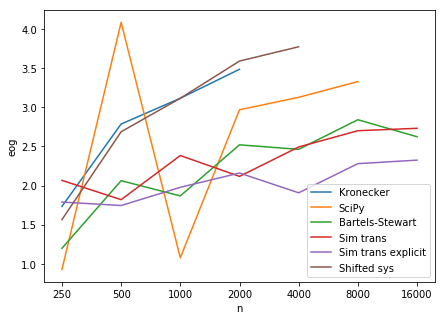
\includegraphics[scale=.6]{img/direct.png}
\caption{The experimental orders of growth of the direct methods.}
\label{fig:direct}
\end{figure}

For the iterative methods, using the Kronecker product and solving using \texttt{sparse.linalg.cg} was faster and, for larger problem sizes, computed a solution in less iterations than the preconditioned MCG and the shifted system method. For $n=16000$, \texttt{sparse.linalg.cg} resulted in a memory error whereas the shifted system method resulted in a timing error. This shows that whilst \texttt{sparse.linalg.cg} is faster, the shifted system method is more memory efficient. The other two iterative methods that were implemented, the gradient based algorithm and the MCG, took too long to compute a solution. A comparison of the eogs of the iterative methods is given in Figure \ref{fig:iterative}.

\begin{figure}[H]
\centering
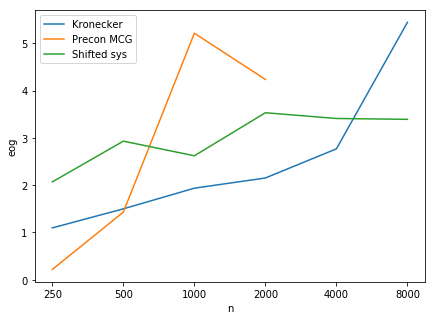
\includegraphics[scale=.6]{img/iterative.png}
\caption{The experimental orders of growth of the iterative methods.}
\label{fig:iterative}
\end{figure}

Of all the methods implemented, we can see that the similarity transformation method, explicitly calculating the eigenpairs and taking advantage of the fact that $P$ is unitary, was the fastest method for large $n$ with the lowest time complexity. We have therefore shown that, by forming this problem as a Sylvester equation and taking advantage of the problem's structure, we were able to dramatically improve performance in terms of both memory requirements and time taken to compute a solution. A comparison of the eogs of all methods is given in Figure \ref{fig:methods}.

\begin{figure}[H]
\centering
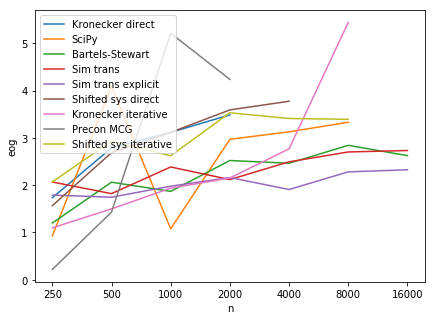
\includegraphics[scale=.6]{img/methods.png}
\caption{The experimental orders of growth of all methods implemented.}
\label{fig:methods}
\end{figure}

\newpage

\section{Uncertainty}
This section explores methods for solving PDEs with uncertain input. Uncertainty can arise in PDEs if, for example, coefficients, boundary conditions or initial conditions are unknown. There are many applications from which uncertainy can arise in PDEs, for example in heat and sound propagation \cite{Swanson}, \cite{Pryhara}, fluid-dynamics \cite{Breit}, \cite{Holm}, cell biology \cite{Bressloff}, population biology \cite{Edwards} and mathematical finance \cite{Shreve03}, \cite{Shreve04}. A solution to dealing with uncertainty is to model unknown parameters as random variables. Appropriate methods can then be used to solve the problem. 

\subsection{Single Parameter}
The simplest way to introduce uncertainty into a PDE is by introducing a single unknown parameter. We define the spatial domain $\mathcal{D}$ as $\mathcal{D} = \{(x,y) : 0 \leq x \leq 1, \; 0 \leq y \leq 1 \}$, and let $\Omega$ denote the sample space. We can introduce an unknown coefficient $\varepsilon(\omega)$, where $\omega \in \Omega$ denotes dependence on a random variable and $\varepsilon: \Omega \rightarrow \mathbb{R}$ is uniformly distributed over the interval $[1,3]$. Let $u(x,y,\varepsilon) = \sin(\pi x)\sin(\pi y) + \varepsilon \sin(3 \pi x) \sin(5 \pi y)$ be the exact solution of the equation:
\begin{alignat}{1}
-\varepsilon u_{xx} -\varepsilon u_{yy} = {}& f \quad \text{ on } \mathcal{D} \times \Omega \nonumber \\
u = {}& 0 \quad \text{ on } \partial \mathcal{D} \times \Omega
\end{alignat}

which gives:
\begin{equation}
\begin{split}
u_{xx} = -\pi^2 \sin(\pi x) \sin(\pi y) - 9\pi^2 \varepsilon \sin(3\pi x) \sin(5\pi y) \\
u_{yy} = -\pi^2 \sin(\pi x) \sin(\pi y) - 25\pi^2 \varepsilon \sin(3\pi x) \sin(5\pi y) \\
\implies f = 2\pi^2 \varepsilon \sin(\pi x) \sin(\pi y) + 34\pi^2 \varepsilon^2 \sin(3\pi x) \sin(5\pi y)
\end{split}
\end{equation}

The equation to be solved is therefore:
\begin{alignat}{1}
- \varepsilon u_{xx} - \varepsilon u_{yy} = {} & 2\pi^2 \varepsilon \sin(\pi x) \sin(\pi y)+ 34 \pi^2 \varepsilon^2 \sin(3 \pi x) \sin(5 \pi y) \quad \text{ on } \mathcal{D} \times \Omega \nonumber \\
u = {} & 0 \quad \text{ on } \partial \mathcal{D} \times \Omega
\end{alignat}
As $\varepsilon$ is unknown, the exact solution to (4.3) cannot be obtained and therefore computed solutions to (4.3) cannot be compared to the actual solution. Instead, certain quantities of interest can be computed using the probability density function $\rho(\omega)$ of $\varepsilon$. Firstly, the expectation $\mathbb{E}[u]$ can be computed as:
\begin{equation}
\mathbb{E}[u] = \int_{\Omega} u(x,y,\varepsilon) \rho(\omega) d \omega
\end{equation}
The variance $\text{Var}[u]$ can also be computed as:
\begin{equation}
\text{Var}[u] = \int_{\Omega} \left(u(x,y,\varepsilon) - \mathbb{E}[u] \right)^2 \rho(\omega) d \omega
\end{equation}
and the standard deviation as $\text{Std}[u] = \sqrt{\text{Var}[u]}$. As $\varepsilon$ is uniformly distributed over the interval $[1,3]$, it has a probability distribution function:
\begin{equation}
\rho(\omega) = \frac{1}{2}
\end{equation}
The expectation is therefore:
\begin{equation}
\begin{split}
\mathbb{E}[u] = & \frac{1}{2} \int_{1}^3 \sin(\pi x)\sin(\pi y) + \varepsilon \sin(3 \pi x) \sin(5 \pi y) d \omega \\
= & \frac{1}{2} \left[\varepsilon \sin(\pi x) \sin(\pi y) + \frac{\varepsilon^2}{2} \sin(3 \pi x) \sin(5 \pi y)\right]_{1}^{3} \\
= & \sin(\pi x) \sin(\pi y) + 2 \sin(3\pi x)\sin(5\pi y)
\end{split}
\end{equation}
and the variance is:
\begin{equation}
\begin{split}
\text{Var}[u] = & \frac{1}{2} \int_{1}^3 \Big( \big( \sin(\pi x) \sin(\pi y) + \varepsilon \sin(3 \pi x) \sin(5 \pi y) \big) \\
& - \big(\sin(\pi x) \sin(\pi y) + 2\sin(3\pi x)\sin(5\pi y) \big) \Big)^2 d \omega \\
= & \frac{1}{2} \int_{1}^3 (\varepsilon-2)^2 \sin^2 (3 \pi x) \sin^2 (5 \pi y) d \omega \\
= & \frac{1}{2} \left[ \left( \frac{\varepsilon^3}{3}-2\varepsilon^2 + 4\varepsilon \right) \sin^2 (3 \pi x) \sin^2 (5 \pi y) \right]_{1}^3 \\
= & \frac{1}{3} \sin^2 (3 \pi x) \sin^2 (5 \pi y)
\end{split}
\end{equation}

which gives the standard deviation as $\text{Std}[u] = \frac{1}{\sqrt{3}} \sin(3 \pi x) \sin(5 \pi y)$. Methods can now be used that compute approximate solutions to these quantities of interest, which can then be compared to the known quantities above to give an estimation of the error. In this section we choose the expectation to measure the error. A plot of the expectation, with $n=1000$, is given in Figure \ref{fig:single}. As can be seen from this figure, the expectation is more complex than the exact solution in the previous section.

\begin{figure}[H]
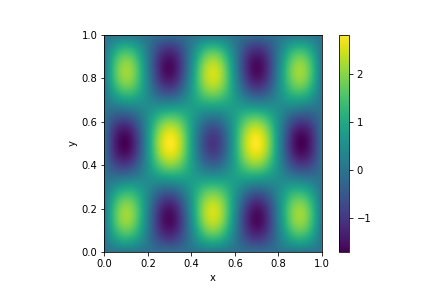
\includegraphics[scale=.7]{img/single.png}
\centering
\caption{Plot of the expectation of the single random parameter problem with $n=1000$.}
\label{fig:single}
\end{figure} 

Throughout this section the following parameters will be used to evaluate performance:
\begin{itemize}
\item $n$: The number of unknowns in each direction - the total number of unknowns is $n^2$. As before, the mesh will be continually refined by a factor of $\frac{1}{2}$ until either the time limit is reached or a memory error occurs, with the starting value as $n=125$.
\item Time(s): The time taken in seconds for the method to compute a solution to the problem. In this section we will increase the maximum time allowed to 12000 seconds. 
\item $|| \mathbb{E}[u] - \mu ||_{L^\infty} $: Defined similarly to the previous section, however we now measure the maximum difference between the expectation and the computed mean solution, that is:
 \[ || \mathbb{E}[u] - \mu ||_{L^\infty} = \text{max}_{ij} \big| \mathbb{E}[u](x_i,y_j) - \mu_{ij} \big| \]
where $\mathbb{E}[u]$ denotes the expectation and $\mu$ denotes the computed mean solution.
\item $\left|\left| \mathbb{E}[u] - \mu \right|\right|_{L^2}$: Defined similarly to the previous section, however we now measure the average difference between the expectation and the computed mean solution, that is:
\[ \left| \left| \mathbb{E}[u] - \mu \right| \right|_{L^2} = \sqrt{h^2 \sum \big| \mathbb{E}[u](x_i,y_j) - \mu_{ij} \big|^2} \]
\item The eoc and eog are defined as in the previous section, that is:
\[ \text{eoc}(i) = \frac{\log(\nicefrac{E_i}{E_{i-1}})}{\log(\nicefrac{h_i}{h_{i-1}})} \]
where $E_i$ is the error (chosen here as $|| \mathbb{E}[u] - \mu ||_{L^\infty}$) and $h_i$ is the mesh size at level $i$,
\[ \text{eog}(i) = \frac{\log(\nicefrac{t_{i}}{t_{i-1}})}{\log(\nicefrac{n_{i}}{n_{i-1}})} \]
where $t_i$ is the total execution time and $n_i$ is the problem size at level $i$.
\end{itemize}
Any additional parameters which relate to the specific methods implemented will be specified. 

\subsubsection{Monte Carlo}
A simple way of solving (4.4) is to use the Monte Carlo method. The Monte Carlo method takes $M$ random samples of $\varepsilon$ over its range, and then solves the PDE for each of these samples. Firstly, we discretise the domain of the PDE using the centred finite difference approximations to form (4.3) as a matrix equation:
\begin{equation}
TU + UT = F
\end{equation}
with $T = -\frac{\varepsilon}{h^2} \text{tridiag}(1,-2,1)$, $U_{ij} = u(x_i, y_j)$ and $F_{ij} = 2\pi^2 \varepsilon \sin(\pi x_i) \sin(\pi y_j)+ 34 \pi^2 \varepsilon^2 \sin(3 \pi x_i) \sin(5 \pi y_j)$. We can now use the most effective method from Section 3 as a `black box' strategy. Once solved, the mean solution can be calculated as:
\begin{equation}
\mu = \frac{1}{M} \sum_{i=1}^M u_h (x, y, \varepsilon)
\end{equation}
where $M$ is the number of samples used in the Monte Carlo method and $u_h$ is the solution obtained from the finite difference method using a mesh of size $h$. Similarly, the variance can be computed as:
\begin{equation}
\sigma^2 = \frac{1}{M-1}\sum_{i=1}^M (u_h - \mu)^2
\end{equation}
and the standard deviation is $\sigma$. We can then compare these quantities to the known values previously computed to calculate the error.

As noted in \cite{Bishop}, for the error to converge to 0 the mesh size must be decreased as the number of samples is increased. This is because the error depends both on the mesh size and the number of samples. By changing only one of these factors the method will be converging to the error of the factor that is not being changed, rather than to 0. It is also worth noting that as the solution and therefore the error is dependent on a random variable, the error itself is a random variable and therefore an increase in the number of samples does not guarantee a reduction in error. However, the law of large numbers tells us that by taking more and more samples the error in expectation should decrease.

It is well known that the convergence rate of the Monte Carlo method is proportional to $\frac{1}{\sqrt{M}}$ \cite{Kalos}. We should therefore expect the eoc to be much lower than the eoc of the methods in the previous section. The order of growth depends on both the method chosen to solve the PDE for each sample and the rate at which the samples are increased at each level. We will choose to increase the number of samples by a factor of 4 as the mesh size is halved to allow for a wide range of sample sizes to be tested without having to increase the execution time by too much.

We choose to use the similarity transformation method from the previous section, calculating the eigenpairs explicity, to solve the PDE for each sample. This method can be used because multiplying a matrix by a constant has the effect of changing the matrix's eigenvalues by that constant while the eigenvectors remain unchanged. This is easy to see by multiplying a general matrix $A$ with eigenvalue $\lambda$ and eigenvector $v$ by a constant $\alpha$, as we have $Av = \lambda v \implies \alpha A v = \alpha \lambda v$. Since we already know the eigenpairs of $-\frac{1}{h^2} \text{tridiag}(1,-2,1)$ from the previous section and $\varepsilon$ is sampled, we can easily obtain the eigenpairs of $T$. 

To ensure that the results obtained by this method are reproducible, each sampled $\varepsilon$ will be seeded. This means that the error computed by this method will be dependent on the seed chosen. To counter this, the computation will be repeated with 10 different seeds (the integers from $0, \dots, 9$) and the error and time taken will be taken as the average error and time taken from each seed used.

Results using the Monte Carlo method, with a single uncertain parameter, are given in Table \ref{table:monte carlo}. The errors here are clearly much bigger than the errors in the previous section, and decrease at a much slower rate, as exemplified by the eoc. The eog here is approximately of order 4, much higher than using the similarity transformation method on the PDE without randomness. This is not surprising as the method needs to be repeated $M$ times, which also causes a dramatic increase in the time taken to compute a solution, as now we are only able to solve the problem for up to $n=2000$ before the (increased) time limit is reached.  
\begin{table}[H]
\centering
\begin{tabular}{|c|c|c|c|c|c|c|}
\hline
$n$ & $M$ & Time(s) & $|| \mathbb{E}[u] - \mu ||_{L^{\infty}}$ & $|| \mathbb{E}[u] - \mu ||_{L^{2}}$ & eoc & eog \\
\hline
125 & 10 & 0.15167 & 0.17459 & 0.087277 & - & - \\
250 & 40 & 2.2733 & 0.10691 & 0.053455 & 0.71166 & 3.9058 \\
500 & 160 & 38.146 & 0.049836 & 0.024919 & 1.1043 & 4.0687 \\
1000 & 640 & 628.53 & 0.017791 & 0.0088953 & 1.4882 & 4.0424 \\
2000 & 2560 & 10755 & 0.0068244 & 0.0034121 & 1.3834 & 4.0969 \\
\cline{2-7}
4000 & \multicolumn{6}{c|}{Time limit reached} \\
\hline
\end{tabular}
\captionsetup{justification=centering}
\caption{Results using the Monte Carlo method with a single uncertain parameter, using the similarity transformation method calculating the eigenpairs explicitly to solve each PDE.}
\label{table:monte carlo}
\end{table}


\subsubsection{Stochastic Galerkin}
The stochastic Galerkin method uses the properties of orthogonal polynomials to produce a functional approximation to the solution of a PDE with an uncertain coefficient. It does this by using a Galerkin projection to ``discretise the random dimensions to allow computation'' \cite{Paul}. 

A set of polynomials $\{\Psi_n(\varepsilon), n \in \mathbb{N}\}$, where $\Psi_n(\varepsilon)$ is a polynomial of exact degree $n$, is orthogonal if it satisfies the orthogonality condition:
\begin{equation}
\int_{\Omega} \Psi_n(\varepsilon) \Psi_m(\varepsilon) w(\varepsilon) d\varepsilon = h_n \delta_{nm}, \quad n,m \in \mathbb{N}
\end{equation} 
where $\Omega$ represents the support of $\{\Psi_n\}$ (the subset of the domain containing elements not mapped to zero), $w(\varepsilon)$ is a weight function, $h_n$ are non-zero constants and $\delta_{nm}$ is the Kronecker delta ($\delta_{nm} = 1$ for $n=m$ and $0$ otherwise). This condition is used to define the inner product of two polynomial functions, $f(\varepsilon)$ and $g(\varepsilon)$, with respect to a weight function $w(\varepsilon)$, as:
\begin{equation}
\langle f, g \rangle = \int_{\Omega} f(\varepsilon)g(\varepsilon)w(\varepsilon) d\varepsilon
\end{equation}

As noted in \cite{Xiu}, certain classes of orthogonal polynomials have the exact same weight function as the probability distribution functions of certain random variables. This property allows the solution $u$ of a random PDE to be approximated via a truncated polynomial chaos expansion using the probability distribution function of the random variable as:
\begin{equation}
u(x,y,\varepsilon) = \sum_{k=0}^P u_k(x,y) \Psi_k(\varepsilon)
\end{equation}
which can then be substituted into the PDE. Here $P+1 = \frac{(K+R)!}{K!R!}$, where $R$ is the number of random variables and $K$ is a convergence parameter to be chosen. In this case we have $R=1 \implies P+1=\frac{(K+1)!}{K!}\implies P=K$.

%Any random quantities can be represented via a Karhunen-Loeve expansion as:
%\begin{equation}
%\alpha =  \bar{\alpha} + \sum_{k=1}^{Q}  \sqrt{\lambda_k} \phi_k \varepsilon_k
%\end{equation}
%for a spatially varying random field $\alpha$ with mean $\bar{\alpha}$, where $\lambda_k$ and $\phi_k$ are the eigenvalues and eigenfunctions of the covariance function $C_\alpha$.


A Galerkin projection is then performed on the PDE by multiplying it by $\Psi_k$ for $k=0, \dots, P$ and taking the inner product, which gives a system of coupled deterministic differential equations, which can then be discretised and solved via, for example, the finite difference method. The resulting solution matrix will be of size $n^2 \times (P+1)$, where $n$ is the number of unknowns in each direction of the mesh and $P$ is defined as above. The mean and variance are then computed as:
\begin{equation}
\mu = u_0
\end{equation}
\begin{equation}
\sigma^2 = \sum_{k=1}^P u_k^2 \mathbb{E}[\Psi_k^2]
\end{equation}

For equation (4.4), $\varepsilon$ is uniformly distributed over the interval $[1,3]$. We introduce the substitution $\varepsilon = \varepsilon_0 + 2$ into this equation, with $\varepsilon_0 \sim u(-1,1)$, so that the random variable in the equation has zero expectation. We then use the Legendre polynomials, which have the same weighting function as the probability density function of the uniform distribution, to solve the equation. They are defined as the polynomials which solve the equation:
\begin{equation}
\frac{d}{d\varepsilon} \left[ (1-\varepsilon^2) \frac{d\Psi_n(\varepsilon)}{d\varepsilon} \right] + n(n+1) \Psi_n(\varepsilon) = 0 
\end{equation}
The SciPy library has a built in function, \texttt{special.legendre}, for calculating Legendre polynomials, which will be used along with the numerical integration function \texttt{integrate.quad}, to evaluate the inner product. We now omit the notation $\Psi_k (\varepsilon)$ to denote dependence on $\varepsilon$ and simply write $\Psi_k$.

From equation (4.3), we now have:
\begin{equation}
(\varepsilon_0+2)(- u_{xx} - u_{yy}) = f
\end{equation}
with $f = 2\pi^2 (\varepsilon_0 +2) \sin(\pi x) \sin(\pi y)+ 34 \pi^2 (\varepsilon_0 + 2)^2 \sin(3 \pi x) \sin(5 \pi y)$. Approximating the solution $u$ using a polynomial chaos expansion and substituting gives:
\begin{equation}
(\varepsilon_0 + 2) \sum_{i=0}^P (-(u_i)_{xx} -(u_i)_{yy}) \Psi_i = f
\end{equation}

Finally, we multiply both sides by $\Psi_k$ and take the inner product, giving:
\begin{equation}
\sum_{i=0}^P (-(u_i)_{xx} -(u_i)_{yy}) \langle \Psi_k (\varepsilon_0 + 2) \Psi_i \rangle = \langle f \Psi_k \rangle
\end{equation}
for $k = 0, \dots, P$, where:
\begin{equation}
\langle f \Psi_k \rangle = 2\pi^2 \sin(\pi x) \sin(\pi y) \langle \Psi_k (\varepsilon_0 + 2) \rangle
+ 34 \pi^2 \sin(3 \pi x) \sin(5 \pi y) \langle \Psi_k (\varepsilon_0 + 2)^2 \rangle
\end{equation}

The uncertainty has been removed from this PDE and we now have a system of coupled deterministic differential equations, which can be solved for $u$. The next step is to rewrite (4.20) in a form that can be easily solved.

Firstly, we can use the finite difference method to discretise the system in space and represent the unknowns $u_i$ as a single vector. Let $L$ be the five-point finite difference stencil, that is, $L= I \otimes T + T \otimes I$, where $T=-\frac{1}{h^2} \text{tridiag}(1,-2,1)$ for grid spacing $h$ and $I$ is the identity matrix. We can then represent the unknowns as:
\begin{equation}
Lu_i = - (u_i)_{xx} - (u_i)_{yy}
\end{equation}
for $i=0,\dots,P$, where $L$ has dimension $n^2 \times n^2$ and $u_i$ is a vector of length $n^2$. We can also represent the inner product on the left-hand side as a $(P+1) \times (P+1)$ matrix:
\begin{equation}
P_{ij} = \langle \Psi_i (\varepsilon_0 + 2) \Psi_j \rangle
\end{equation}
for $i,j = 0,\dots,P$. Finally, we represent the right-hand side of the system as a $n^2 \times (P+1)$ matrix:
\begin{equation}
F_{k} = 2\pi^2 \sin(\pi x_i)\sin(\pi y_j) \langle \Psi_k (\varepsilon_0 + 2) \rangle + 34\pi^2 \sin(3\pi x_i) \sin(5\pi y_j) \langle \Psi_k (\varepsilon_0 + 2)^2 \rangle
\end{equation}
where $k = 0, \dots, P$ represents the columns (the random discretisation) and $i,j = 1, \dots, n$ represent the rows (the vectorised spatial dicretisation). We can now use these matrices to rewrite (4.20) in a form that can be easily solved. When using this method we will choose $K=1 \implies P=1$, as increasing $K$ does not have a significant affect on the error but vastly increases computation time. 

\subsubsection*{Linear System}
The simplest way to solve (4.20) is to form the problem as a linear system. By reshaping $F$ into a vector we can represent the problem in the form:
\begin{equation}
Au = f
\end{equation} 
where $A = P \otimes L$ has dimension $n^2(P+1) \times n^2(P+1)$ and $f = \text{vec}(F)$ and $u$ are vectors of length $n^2(P+1)$. We can now use a standard sparse solver to solve the system. Results using the conjugate gradient method \texttt{sparse.linalg.cg} from the SciPy library, using a convergence tolerance of $10^{-9}$, are given in Table \ref{table:stochastic linear}.

\begin{table}[H]
\centering
\begin{tabular}{|c|c|c|c|c|c|}
\hline
$n$ & Time(s) & $|| \mathbb{E}[u] - \mu ||_{L^{\infty}}$ & $|| \mathbb{E}[u] - \mu ||_{L^{2}}$ & eoc & eog \\
\hline
125 & 0.014717 & 0.0021941 & 0.0010767 & - & - \\
250 & 0.077675 & 0.00055263 & 0.00027120 & 2.0007 & 2.4000 \\
500 & 0.52634 & 0.00013874 & 6.80630 $\times 10^{-5}$ & 1.9997 & 2.7605 \\
1000 & 3.7997 & $3.4817 \times 10^{-5}$ & $1.7049 \times 10^{-5}$ & 1.9974 & 2.8518  \\
2000 & 33.354 & $8.7386 \times 10^{-6}$ & $4.2666 \times 10^{-6}$ & 1.9958 & 3.1339 \\
4000 & 308.21 & $2.2358 \times 10^{-6}$ & $1.0674 \times 10^{-6}$ & 1.9673 & 3.2080 \\
8000 & 3090.0 & $6.4883 \times 10^{-7}$ & $2.6774 \times 10^{-7}$ & 1.7852 & 3.3256 \\
\cline{2-6}
16000 & \multicolumn{5}{c|}{Memory Error} \\
\hline
\end{tabular}
\captionsetup{justification=centering}
\caption{Results using the stochastic Galerkin method with a single uncertain parameter by solving the linear system using \texttt{sparse.linalg.cg}.}
\label{table:stochastic linear}
\end{table}

From these results we can see that the errors here are significantly less than with the Monte Carlo method and the eoc is much closer to 2, especially for $n<8000$. The eog is slightly more than 3, a significant improvement on the Monte Carlo method which had an eog of approximately 4. Furthermore, the time taken taken to compute a solution is clearly much less than with the Monte Carlo method, and we were able to compute a solution for problem sizes up to $n=8000$ before a memory error occurred. It is therefore clear that using this method has a significant advantage over the Monte Carlo method.

\subsubsection*{Matrix Equation}
An alternative approach to solving (4.20) is to rewrite it as a matrix equation, in the form:
\begin{equation}
LXP = F
\end{equation} 
where $u = \text{vec}(X)$ and $L$, $P$ and $F$ are defined as before. 

One way to solve this is by using a variation of the Bartels-Stewart algorithm. The basic idea is the same as the standard Bartels-Stewart algorithm from Section 3.1.2. Firstly, the Schur decomposition of $L$ and $P$ is computed, so that the equation can be transformed into an equivalent upper-triangular system that can be solved element by element. The solution to the original equation is then easily obtained using the solution of the triangular system. The steps of this algorithm are as follows:
\begin{enumerate}
\item Compute the Schur forms $L = U \hat{L} U^*$ and $P = V \hat{P} V^*$, and let $\hat{F} = U^* F V$.
\item Solve $\hat{L} Y \hat{P} = \hat{F}$ for $Y$, where $\hat{L}$ and $\hat{P}$ are upper triangular.
\item Compute solution $X = UYV^*$.
\end{enumerate}
The problem with this method is that the Schur forms in the first step are computed using the QR algorithm. The matrices produced in the decomposition using this algorithm are dense. Therefore a huge amount of memory is required to compute and store the Schur form of $L$ (of size $n^2 \times n^2$), which is impractical even for a relatively small problem size. This method was tested on the problem with $n=125$ and $K=1$, and resulted in a memory error when computing the Schur forms, which confirms that this method is not appropriate for this problem.

Alternatively, we can right multiply by $P^{-1}$ to obtain:
\begin{equation}
LX = FP^{-1}
\end{equation}
The resulting right-hand side is a matrix, meaning \texttt{sparse.linalg.spsolve} can be used to compute a solution\footnote{\texttt{sparse.linalg.cg} cannot be used here as it requires the right-hand side to be a vector, but \texttt{spsolve} can be used when the right-hand side is a matrix.}. Results of doing so are given in Table \ref{table:stochastic matrix}. It is clear from these results that, for problem sizes it is able to solve for, this method takes longer than using the conjugate gradient method on the linear system. The errors here are similar to the errors when solving the linear system. The differences are likely due to using a direct solver rather than an iterative one, which is also likely why, for problem sizes it is able to solve, the eoc is closer to 2 than the previous method. The eog is also slightly better than solving the linear system. For $n=4000$, this method results in a memory error, as \texttt{spsolve} destroys the sparsity of $L$, which significantly increases memory requirements, as previously mentioned.

\begin{table}[H]
\centering
\begin{tabular}{|c|c|c|c|c|c|}
\hline
$n$ & Time(s) & $|| \mathbb{E}[u] - \mu ||_{L^{\infty}}$ & $|| \mathbb{E}[u] - \mu ||_{L^{2}}$ & eoc & eog \\
\hline
125 & 0.059279 & 0.0021941 & 0.0010767 & - & - \\
250 & 0.25614 & 0.00055258 & 0.00027120 & 2.0009 & 2.1113 \\
500 & 1.4756 & 0.00013872 & $6.8063 \times 10^{-5}$ & 1.9998 & 2.5263 \\
1000 & 10.827 & $3.4752 \times 10^{-5}$ & $1.7049 \times 10^{-5}$ & 1.9999 & 2.8753 \\
2000 & 76.430 & $8.6968 \times 10^{-6}$ & $4.2666 \times 10^{-6}$ & 2.0000 & 2.8195 \\
\cline{2-6}
4000 & \multicolumn{5}{c|}{Memory Error} \\
\hline
\end{tabular}
\captionsetup{justification=centering}
\caption{Results using the stochastic Galerkin method with a single uncertain parameter by solving the matrix equation using \texttt{sparse.linalg.spsolve}.}
\label{table:stochastic matrix}
\end{table}


\subsubsection*{Sylvester Equation}
From \cite{Powell}, we can instead rewrite the problem as an alternative matrix equation in the form:
\begin{equation}
2LXG_0 + LXG_1 = F
\end{equation}
where $u = \text{vec}(X)$, $(G_0)_{ij} = \langle \Psi_i \Psi_j \rangle$ and $(G_1)_{ij} = \langle \Psi_i \varepsilon_0 \Psi_j \rangle$. By left and right multiplying by $L^{-1}$ and $G_0^{-1}$ respectively, we obtain the equation in Sylvester form:
\begin{equation}
AX + XB = C
\end{equation}
where $A = L^{-1}2L$, $B = G_1 G_0^{-1}$ and $C = L^{-1} F G_0^{-1}$. This can now be solved using any of the methods from Section 3, assuming that they can be adapted for sparse matrices. Computing $L^{-1}$ directly is very expensive and memory inefficient, as it has large dimension and although $L$ is sparse its inverse, in general, will not be. We do not, however, need to compute $L^{-1}$ directly, we just need its effect on the equation. The matrix $A$ is easily computed as $L^{-1}2L = 2L^{-1}L = 2I$. To compute $C$, we form the linear system:
\begin{equation}
(L \otimes I)\text{vec}(C) = \text{vec}(FG_0^{-1})
\end{equation}
where $I$ is the identity matrix of dimension $(P+1)$. We can then solve for $C$ and reshape it back into a vector, which vastly speeds up computation time and drastically reduces memory requirements. The eigenvalues and eigenvectors of $A$ are simply 2 and the columns of the identity matrix, respectively. As $B$ is a square matrix with dimension $(P+1)=2$ (as we have set $P=1$), computing the eigenpairs of $B$ will be cheap and approximating them will not have a large impact on the error. We can therefore use \texttt{numpy.linalg.eig} to calculate the eigenpairs.

Results using the conjugate gradient method \texttt{sparse.linalg.cg}, with a convergence tolerance of $10^{-9}$ to solve for $C$ and the similarity transformation method to solve for $X$, are given in Table \ref{table:stochastic sylvester}.

\begin{table}[H]
\centering
\begin{tabular}{|c|c|c|c|c|c|c|}
\hline
$n$ & $K$ & Time(s) & $|| \mathbb{E}[u] - \mu ||_{L^{\infty}}$ & $|| \mathbb{E}[u] - \mu ||_{L^{2}}$ & eoc & eog \\
\hline
125 & 1 & 0.011544 & 0.0021941 & 0.0010767 & - & - \\
250 & 1 & 0.032874 & 0.00055258 &  0.00027120 & 2.0009 & 1.5098 \\
500 & 1 & 0.11274 & 0.00013872 & $6.8063 \times 10^{-5}$ & 1.9998 & 1.7780 \\
1000 & 1 &  0.70258 & $3.4752 \times 10^{-5}$ & $1.7049 \times 10^{-5}$ & 1.9999 & 2.6397 \\
2000 & 1 & 5.8607 & $8.6968 \times 10^{-6}$ & $4.2666 \times 10^{-6}$ & 2.0000 & 3.0603 \\
4000 & 1 & 52.552 & $2.1753 \times 10^{-6}$ & $1.0672 \times 10^{-6}$ & 2.0000 & 3.1646 \\
8000 & 1 & 587.73 & $5.4395 \times 10^{-7}$ & $2.6686 \times 10^{-7}$ & 2.0001 & 3.4833 \\
\cline{2-7}
16000 & \multicolumn{6}{c|}{Memory Error} \\
\hline
\end{tabular}
\captionsetup{justification=centering}
\caption{Results using the stochastic Galerkin method with a single uncertain parameter by solving the Sylvester equation using \texttt{sparse.linalg.cg} and the similarity transformation method.}
\label{table:stochastic sylvester}
\end{table}

From these results we can see that, in terms of timing, errors and the eoc, solving this problem as a Sylvester equation is faster and more efficient than solving it as a linear system or alternative matrix equation. The eog here is less than the eog when solving it as a linear system for $n<8000$, and then only slightly higher when $n=8000$. This could be explained by the fact that it is solving two problems (solving for $C$ and then for $X$) rather than just one, and therefore the cost increases when $n$ is large. As with solving the linear system, when $n=16000$ solving the system in this form resulted in a memory error. 

We have now shown that the stochastic Galerkin method significantly outperforms the Monte Carlo method in the single parameter case. We have also shown that forming the stochastic Galerkin problem as a Sylvester equation has significant advantage compared to forming the problem as a linear system or alternative matrix equation. We now move on to introduce multiple unknown parameters into the problem.

\newpage

\subsection{Multiple Parameters}
Multiple unknown parameters can be introduced into the PDE, which makes it significantly harder to solve accurately and efficiently. Each parameter is modelled as an independent random variable. Let $\varepsilon$ now be defined as:
\begin{equation}
\varepsilon = \sum_{p,q = 1}^N 2^{-(p+q)} \varepsilon_{pq} \sin(p \pi x) \sin(q \pi y)
\end{equation}
with $\varepsilon_{pq} \sim u(-1,1)$. Then let $u = \sin(\pi x)\sin(\pi y) + \varepsilon$ be the solution of the PDE:
\begin{alignat}{1}
-\varepsilon u_{xx} -\varepsilon u_{yy} = {}& f \quad \text{ on } \mathcal{D} \times \Omega \nonumber \\
u = {}& 0 \quad \text{ on } \partial \mathcal{D} \times \Omega
\end{alignat}
which gives:
\begin{equation}
\begin{split}
u_{xx} &= -\pi^2 \sin(\pi x)\sin(\pi y) - \sum_{p,q=1}^N 2^{-(p+q)} p^2 \pi^2 \varepsilon_{pq} \sin(p\pi x)\sin(q\pi y) \\
u_{yy} &= -\pi^2 \sin(\pi x)\sin(\pi y) - \sum_{p,q=1}^N 2^{-(p+q)} q^2 \pi^2 \varepsilon_{pq} \sin(p\pi x)\sin(q\pi y) \\
\implies f &= \varepsilon \Big(2\pi^2 \sin(\pi x) \sin(\pi y) + \pi^2 \sum_{p,q=1}^N 2^{-(p+q)} (p^2 + q^2) \varepsilon_{pq} \sin(p \pi x)\sin(q \pi y) \Big) \\
%&= \Big(\sum_{p,q=1}^N 2^{-(p+q)} \varepsilon_{pq} \sin(p\pi x)\sin(q\pi y) \Big)
%\\ &\times \Big(2\pi^2 \sin(\pi x) \sin(\pi y) + \pi^2 \sum_{p,q=1}^N 2^{-(p+q)} (p^2 + q^2) \varepsilon_{pq} \sin(p \pi x)\sin(q \pi y) \Big)
\end{split}
\end{equation}
There are now $N^2$ random variables in the equation. We now calculate the expectation of $u$. Instead of evaluating the integral explicitly to obtain the expectation, a simpler way is to calculate it as:
\begin{equation}
\mathbb{E}[u] = \mathbb{E}[\sin(\pi x)\sin(\pi y)] + \mathbb{E}\left[\sum_{p,q=1}^N -2^{p+q} \varepsilon_{pq} \sin(\pi x)\sin(\pi y) \right]
\end{equation}
As all $\varepsilon_{pq}$ are uniformly distributed between -1 and 1, they have 0 expectation and so the expectation of $u$ is simply:
\begin{equation}
\mathbb{E}[u] = \sin(\pi x)\sin(\pi y)
\end{equation}
As in the single parameter case, we can now use methods to calculate an approximation of the expectation and then compare them to the known expectation to give a measure of error. Note that this expectation is the same as the exact solution in Section 3. A plot of the expectation, with $n=1000$, is given in Figure \ref{fig:multiple}.

\begin{figure}[H]
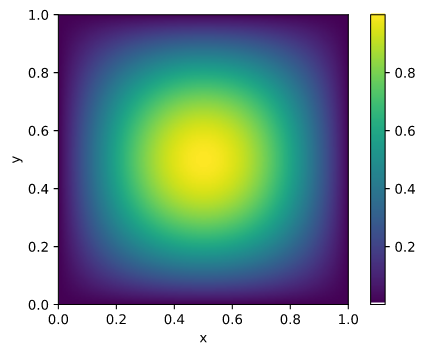
\includegraphics[scale=.5]{img/solution2.png}
\centering
\caption{Plot of the expectation of the multiple random parameter problem with $n=1000$.}
\label{fig:multiple}
\end{figure} 

\subsubsection{Monte Carlo}
As in the single parameter case, we can use the Monte Carlo method to solve (4.32). We simply take $M$ random samples of each $\varepsilon_{pq}$ and solve the PDE for each of these samples. The expectation is then calculated as the mean solution. Firstly, we discretise the spatial dimensions using the centred finite difference approximations to obtain:
\begin{equation}
TU + UT = F
\end{equation}
with $T= -\frac{\varepsilon}{h^2}\text{tridiag}(1,-2,1)$, $U_{ij} = u(x_i,y_j)$ and: 
\[F_{ij}=\varepsilon \Big(2\pi^2 \sin(\pi x) \sin(\pi y) + \pi^2 \sum_{p,q=1}^N 2^{-(p+q)} (p^2 + q^2) \varepsilon_{pq} \sin(p \pi x)\sin(q \pi y) \Big) \]

We can now choose the best method from Section 3 to solve (4.36) for each sample. As with the single parameter Monte Carlo method, we use the similarity transformation method, explicitly calculating the eigenpairs. 

Similarly to Section 4.1.1, the number of samples will be increased by a factor of 4 as the mesh size is halved. We will vary $N$ to see how this affects the error. Also, each test will be repeated with 10 different seeds and averaged to ensure that the result is not dependent on the seed. 

One thing to note is that the summation of $\varepsilon_{pq}$ depends on the spatial dimensions $x$ and $y$. In other words, the summation changes and therefore needs to be recalculated depending on the grid point. Because of this, constructing the problem will take an increasingly long time as both $n$ and $N$ are increased. However, we are only interested in how long this method takes to solve the problem and so we will only time how long this method takes to compute a solution. 

Results of this method are given in Table \ref{table:monte carlo multiple}. The first thing to note is that the errors here start off smaller than for the single parameter Monte Carlo case. However, this is a consequence of the expectation rather than the method, as clearly the expectation is simpler in this case than in the single parameter case. We can see from both the errors and the eoc that the errors are decreasing at a slower rate than the single parameter case as the problem size and number of samples are increased, as there is more variation in the solution than in the single parameter. We can also see that the time taken for each problem size is approximately the same regardless of the value of $N$, which is not surprising as the method is solving the same number of PDEs for each problem size. This also explains why the eog is approximately the same for different problem sizes for each $n$.

\begin{table}[H]
\centering
\begin{tabular}{|c|c|c|c|c|c|c|c|}
\hline
$N$ & $n$ & $M$ & Time(s) & $|| \mathbb{E}[u] - \mu ||_{L^{\infty}}$ & $|| \mathbb{E}[u] - \mu ||_{L^{2}}$ & eoc & eog \\
\hline
\multirow{4}{*}{2} & 125 & 10 & 0.13827 & 0.097171 & 0.039979 & - & - \\
& 250 & 40 & 2.1282 & 0.050053 & 0.020736 & 0.96259 & 3.9441 \\
& 500 & 160 & 40.034 & 0.036890 & 0.017075 & 0.44150 & 4.2335 \\
& 1000 & 640 & 580.94 & 0.032707 & 0.016318 & 0.17388 & 3.8591 \\
\hline
\multirow{4}{*}{4} & 125 & 10 & 0.13955 & 0.088060 & 0.035807 & - & - \\
& 250 & 40 & 2.1259 & 0.081807 & 0.036437 & 0.10688 & 3.9292 \\
& 500 & 160 & 39.872 & 0.057317 & 0.026807 & 0.51474 & 4.2292 \\
\cline{4-8}
& 1000 & 640 & \multicolumn{5}{c|}{Time limit reached} \\
\hline
\multirow{4}{*}{8} & 125 & 10 & 0.13894 & 0.10960 & 0.044472 & - & - \\
& 250 & 40 & 2.2092 & 0.054684 & 0.022630 & 1.0088 & 3.9910 \\
& 500 & 160 & 34.502 & 0.047838 & 0.021733 & 0.19352 & 3.9651 \\
\cline{4-8}
& 1000 & 640 & \multicolumn{5}{c|}{Time limit reached} \\
\hline
\end{tabular}
\captionsetup{justification=centering}
\caption{Results using the Monte Carlo method with multiple uncertain parameters, using the similarity transformation method calculating the eigenpairs explicitly to solve each PDE.}
\label{table:monte carlo multiple}
\end{table}

\subsubsection{Stochastic Galerkin}
We can use the stochastic Galerkin method to solve the problem with multiple uncertain parameters, however it is now significantly more complex. We begin with:
\begin{equation}
\varepsilon(-u_{xx} - u_{yy}) = f
\end{equation}
with $\varepsilon$ and $f$ defined as above. The first step is to approximate the solution $u$ using a polynomial chaos expansion, giving:
\begin{equation}
\varepsilon \sum_{i=0}^P (-(u_i)_{xx} - (u_i)_{yy}) \Psi_i = f
\end{equation}
with $P+1 = \frac{(K+R)!}{K!R!}$ where $R$ is the number of random variables and $K$ is a convergence parameter to be chosen. In this case we have $R = N^2 \implies P=\frac{(K+N^2)!}{K!N^2!} - 1$. Here $\Psi$ now denotes the $N^2$-dimensional Legendre polynomials (as there are $N^2$ random variables), which are calculated by taking the product of one-dimensional Legendre polynomials \cite{Paul}, that is:
\begin{equation}
\Psi_{N^2} (\varepsilon_{11}, \varepsilon_{12}, \dots, \varepsilon_{NN}) = \Psi_{i_{11}} (\varepsilon_{11})  \Psi_{i_{12}} (\varepsilon_{12}) \dots \Psi_{i_{NN}} (\varepsilon_{NN})  
\end{equation}
which has weight function $w(\varepsilon_{11}, \dots, \varepsilon_{NN}) = \frac{1}{2^{N^2}}$. Note that here $i_{11} + i_{12} + \dots + i_{NN} \leq N^2$. Next we multiply by $\Psi_k$ and take the inner product, which gives:
\begin{equation}
\sum_{i=0}^P (-(u_i)_{xx} - (u_i)_{yy}) \langle \Psi_k \varepsilon \Psi_i \rangle = \langle f \Psi_k \rangle
\end{equation}
for $k=0,\dots,P$. Here we have:
\begin{equation}
\langle \Psi_i \varepsilon \Psi_k \rangle = \sum_{p,q=1}^N \langle \Psi_i \varepsilon_{pq} \Psi_k \rangle 2^{-(p+q)} \sin(p\pi x)\sin(q\pi y) 
\end{equation}
and:
\begin{equation}
\langle f \Psi_k \rangle = 2 \pi^2 \sin(\pi x)\sin(\pi y) \sum_{p,q=1}^N \langle \Psi_k \varepsilon_{pq} \rangle 2^{-(p+q)} \sin(p \pi x) \sin(q \pi y)  \nonumber
\end{equation}
\begin{equation}
+ \left(\pi^2 \sum_{p,q=1}^N \langle \Psi_k \varepsilon_{pq} \rangle 2^{-(p+q)} (p^2 + q^2) \sin(p \pi x)\sin(q \pi y) \right) \left(\sum_{p,q=1}^N 2^{-(p+q)} \langle \Psi_k \varepsilon_{pq} \rangle \sin(p \pi x)\sin(q \pi y) \right)
\end{equation}
We now have a deterministic coupled set of differential equations that we can solve. We rewrite (4.40) into a form that can be easily solved. Firstly, we use the finite difference method to discretise in space and represent the unknowns $u_i$ as a single vector:
\begin{equation}
Lu_i = - (u_i)_{xx} - (u_i)_{yy}
\end{equation}
for $i=0,\dots,P$. Next, we represent the inner product on the left-hand side as:
\begin{equation}
P_{ij} = \langle \Psi_i \varepsilon_{pq} \Psi_j \rangle
\end{equation}
for $i,j=0,\dots,P$. We can represent this inner product as a single matrix because each $\varepsilon_{pq}$ is defined on the same interval, or, in other words, changing the values of $p$ and $q$ does not change the value of the inner product. We now represent the summation on the left-hand side as a $n^2 \times n^2$ diagonal matrix $D$, which has entries:
\begin{equation}
D_k = \sum_{p,q=1}^N 2^{-(p+q)} \sin(p \pi x_i) \sin(q \pi y_j)
\end{equation}
on the diagonal, for $k=1,\dots,n^2$ (as $i$ and $j$ run from $i,j=1,\dots,n$). Lastly, we represent the right-hand side of the system as:
\begin{equation}
F_k = 2 \pi^2 \sin(\pi x_i) \sin(\pi y) \sum_{p,q=1}^N \langle \Psi_k \varepsilon_{pq} \rangle 2^{-(p+q)} \sin(p \pi x)\sin(q \pi y) \nonumber
\end{equation}
\begin{equation}
+ \left(\pi^2 \sum_{p,q=1}^N \langle \Psi_k \varepsilon_{pq} \rangle 2^{-(p+q)} (p^2 + q^2) \sin(p \pi x)\sin(q \pi y) \right) \left(\sum_{p,q=1}^N 2^{-(p+q)} \langle \Psi_k \varepsilon_{pq} \rangle \sin(p \pi x)\sin(q \pi y) \right)
\end{equation}
for $k=0,\dots,P$ (the random discretisation) and $i,j=1,\dots,n$ (the vectorised spatial discretisation). We can now proceed with solving the system in a variety of ways. Again we set $K=1 \implies P = \frac{(N^2 + 1)!}{N^2 !} - 1$, as higher values of $K$ do not have a significant impact on the error but vastly increase computation time. As with the multiple parameter Monte Carlo method, we are only interested in the time taken to solve the problem (not construct it) and therefore will only time how long a method takes to compute a solution. Also, we should expect the errors here to be smaller than in the single parameter stochastic Galerkin case as the expectation here is simpler.

\subsubsection*{Linear System}
We can represent (4.40) as a linear system in the form:
\begin{equation}
Au = f
\end{equation}
where $A=\left( P \otimes D \right) \left( I \otimes L \right)$ has dimension $n^2(P+1) \times n^2(P+1)$ and $f = \text{vec}(F)$ and $u$ are vectors of dimension $n^2(P+1)$. Here $I$ is the identity matrix of size $(P+1)$. We can now use a standard sparse solver to solve the system. From this formulation it is not clear that $A$ has symmetric structure and so, instead of using the conjugate gradient method, we use \texttt{sparse.linalg.spsolve} to solve the system. Results of doing so are given in Table \ref{table:galerkin multiple linear}.

We can see from these results that the errors here are much lower than the Monte Carlo method, demonstrating that this method is solving the problem more accurately (and are also lower than in the single parameter stochastic Galerkin case, as expected). The errors are also very close the some of the errors given in Section 3. This is because the expectation is the same as the exact solution in the previous section. 


The errors for $N=2$ are bigger than when $N=4$, and while it is not clear why this is 

unlike the Monte Carlo method, the time taken grows as $N$ is increased, which is not surprising as an increase in $N$ causes an increase in the dimension of $P$ and therefore the problem size grows. 

This method results in a memory error for much lower values of $n$ than the single parameter case as the coefficient matrix $A$ is much less sparse.

\begin{table}[H]
\centering
\begin{tabular}{|c|c|c|c|c|c|c|}
\hline
$N$ & $n$ & Time(s) & $|| \mathbb{E}[u] - \mu ||_{L^{\infty}}$ & $|| \mathbb{E}[u] - \mu ||_{L^{2}}$ & eoc & eog \\
\hline
\multirow{4}{*}{2} & 125 & 1.1174 & $5.4475 \times 10^{-5}$ & $2.7192 \times 10^{-5}$ & - & - \\
& 250 & 7.8475 & $1.6508 \times 10^{-5}$ & $7.8571 \times 10^{-6}$ & 1.7324 & 2.8121 \\
& 500 & 63.485 & $6.9480 \times 10^{-6}$ & $3.0622 \times 10^{-6}$ & 1.2521 & 3.0161 \\
\cline{3-7}
& 1000 & \multicolumn{5}{c|}{Memory Error} \\
\hline
\multirow{4}{*}{4} & 125 & 34.658 & $5.1807 \times 10^{-5}$ & $2.5904 \times 10^{-5}$ & - & - \\
& 250 & 221.33 & $1.3054 \times 10^{-5}$ & $6.5275 \times 10^{-6}$ & 2.0001 & 2.6749 \\
\cline{3-7}
& 500 & \multicolumn{5}{c|}{Memory Error} \\
\hline
\end{tabular}
\captionsetup{justification=centering}
\caption{Results using the stochastic Galerkin method with multiple uncertain parameters to solve a linear system using \texttt{spsolve}.}
\label{table:galerkin multiple linear}
\end{table}

\subsubsection{Matrix Equation}
Unfortunately, in this case we cannot rewrite (4.40) as a Sylvester equation that matches the form of the solvers studied in Section 3. We can, however, rewrite it as an alternative matrix equation. From (4.47) we have:
\begin{equation}
\begin{split}
& (P \otimes D)(I \otimes L) u = \text{vec}(F) \\
& = (PI) \otimes (DL) u = \text{vec}(F) \\
& \implies DL X P = F 
\end{split}
\end{equation}
where $u = \text{vec}(X)$. As in the single parameter case, this could be solved using a variation of the Bartels-Stewart algorithm, however would require a huge amount of memory to compute and store the Schur forms of $DL$. Instead, we multiply by $P^{-1}$ to obtain the matrix equation:
\begin{equation}
DL X = F P^{-1}
\end{equation}
We can now solve this form using \texttt{spsolve}. However, in this case, we should expect to be able to solve the problem for larger problem sizes than when solving the linear system as we have maintained the sparsity of the coefficient matrix. Results of doing so are given in Table \ref{table:galerkin multiple matrix}.

We can see from these results that we are able to solve for much larger problem sizes than when solving the linear system. Also, as $N$ is increased, the increase in time taken to compute a solution is much lower than.

\begin{table}[H]
\centering
\begin{tabular}{|c|c|c|c|c|c|c|}
\hline
$N$ & $n$ & Time(s) & $|| \mathbb{E}[u] - \mu ||_{L^{\infty}}$ & $|| \mathbb{E}[u] - \mu ||_{L^{2}}$ & eoc & eog \\
\hline
\multirow{4}{*}{2} & 125 & 0.057401 & $5.4475 \times 10^{-5}$ & $2.7192 \times 10^{-5}$ & - & - \\
& 250 & 0.29013 & $1.6508 \times 10^{-5}$ & $7.8571 \times 10^{-6}$ & 1.7324 & 2.3376 \\
& 500 & 1.6387 & $6.9480 \times 10^{-6}$ & $3.0622 \times 10^{-6}$ & 1.2521 & 2.4978 \\
& 1000 & 11.469 & $4.9213 \times 10^{-6}$ & $1.9335 \times 10^{-6}$ & 0.49828 & 2.8071 \\
& 2000 & 77.098 & $4.4465 \times 10^{-6}$ & $1.6728 \times 10^{-6}$ & 0.14647 & 2.7490 \\
\cline{3-7}
& 4000 & \multicolumn{5}{c|}{Memory Error} \\
\hline
\multirow{4}{*}{4} & 125 & 0.081032 & $5.1807 \times 10^{-5}$ & $2.5904 \times 10^{-5}$ & - & - \\
& 250 & 0.40200 & $1.3054 \times 10^{-5}$ & $6.5275 \times 10^{-6}$ & 2.0001 & 2.3106 \\
& 500 & 2.1681 & $3.2767 \times 10^{-6}$ & $1.6384 \times 10^{-6}$ & 1.9999 & 2.4312 \\
& 1000 & 13.925 & $8.2082 \times 10^{-7}$ & $4.1041 \times 10^{-7}$ & 2.0000 & 2.6832 \\
& 2000 & 88.442 & $2.0540 \times 10^{-7}$ & $1.0270 \times 10^{-7}$ & 2.0000 & 2.6671 \\
\cline{3-7}
& 4000 & \multicolumn{5}{c|}{Memory Error} \\
\hline
\end{tabular}
\captionsetup{justification=centering}
\caption{Results using the stochastic Galerkin method with multiple uncertain parameters to solve a matrix equation using \texttt{spsolve}.}
\label{table:galerkin multiple matrix}
\end{table}

\newpage

\subsection{Conclusion}

In the single parameter case, we demonstrated that we can firstly form the random PDE as a Sylvester equation and solve it using the Monte Carlo method, that is, solve it using the best solver from Section 3 $M$ times and take the average to obtain the solution. We then showed that we can solve the problem more accurately by using the stochastic Galerkin method, and demonstrated that forming the problem as Sylvester equation in this case can result in increased efficiency compared to both the linear system and alternative matrix equation. For comparison, the eogs of the Monte Carlo method and the stochastic Galerkin method solving different forms of the problem are displayed in Figure \ref{fig:single eogs}.

\begin{figure}[H]
\centering
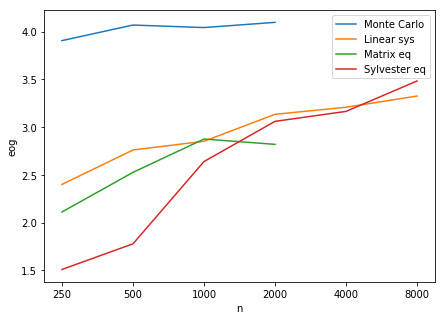
\includegraphics[scale=.6]{img/singleeog.png}
\caption{The experimental orders of growth for the single parameter problem.}
\label{fig:single eogs}
\end{figure}

Similarly, in the multiple parameter case we first formed the random PDE and solved the problem using the Monte Carlo method.

\begin{figure}[H]
\centering
\subfigure[$N=2$]{%
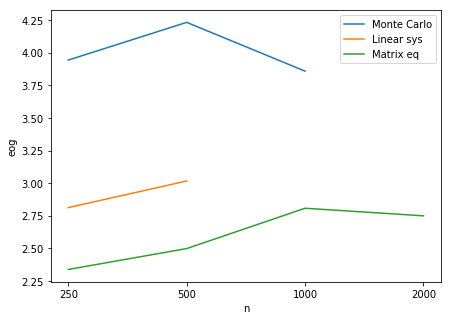
\includegraphics[height=2in]{img/n2.png}}%
\qquad
\subfigure[$N=4$]{%
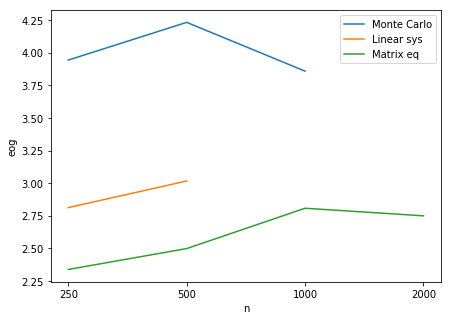
\includegraphics[height=2in]{img/n2.png}}%
\caption{The experimental orders of growth for the multiple parameter problem.}
\label{fig:multiple eogs}
\end{figure}


\newpage

\section{Evaluation}
This section will evaluate whether the project's aims and objectives given in Section 2 were met. It will then go on to state possible project extensions and give a brief conclusion of the success of the project.

\subsection{Aims}
There were two main aims of this project. The first was to study, implement and compare a variety of different methods for solving matrix equations (or more specifically, Sylvester equations). This has clearly been achieved in Section 3, as a number of different methods, both direct and iterative, were studied and analysed, implemented correctly and then compared and evaluated. Also, where possible, general methods were improved upon by taking advantage of the problem's structure. This demonstrates that a deep understanding of what was studied has been achieved.

The other aim of this project was to study methods that are used to solve random PDEs and adapt what had been studied in Section 3 to solve PDEs of this type. This was demonstrated in Section 4, where randomness was introduced into the problem. We firstly studied two methods, Monte Carlo and stochastic Galerkin, which can be used to solve random PDEs. We then used the knowledge that had been gained in the previous section to solve the problem. It is therefore clear that the aims of the project have been met.

\subsection{Extensions}
There are a number of possible extensions that, given additional time, could be applied to this project. These include:
\begin{itemize}
\item Additional matrix solvers: A number of different methods for solving matrix equations were studied, implemented and compared throughout this project. However, if time was not a constraint, additional methods could have been considered, for example the Hessenberg-Schur method \cite{Hessenberg}, the ADI iteration \cite{Simoncini} and a block linear method \cite{Monsalve}.
\item Additional methods for solving random PDEs: In this project we chose to study two general methods for solving random PDEs, Monte Carlo and stochastic Galerkin, so that these could be studied in depth and we could relate them to what was studied in Section 3. Given additional time, other ways of solving random PDEs could have also been studied, for example, reduced basis methods \cite{Powell} and multi-level Monte Carlo methods \cite{Barth}.
\item Random variables with other distributions: The uncertain parameters studied in Section 4 were modelled as random variables with a uniform distribution. A potential extension to this project could be to study the effect of uncertain parameters with other distributions. A few possible examples include the Gaussian, gamma, beta, Poisson, binomial and hypergeometric distributions. See \cite{Xiu} for more details on how these distributions relate to specific classes of orthogonal polynomials.
\item Application problem: The initial plan of the project was to end up with an application problem that could be solved using the knowledge gained from Sections 3 and 4. However, during the project, it was decided to instead analyse the content in Sections 3 and 4 in more detail. A possible extension of this project could be to apply what has been studied to a particular application problem, for example, something similar to \cite{Barreira} involving randomness.
\end{itemize}

\subsection{Personal Reflection}

\subsection{Conclusion}
A comprehensive understanding of methods for solving both matrix equations and random PDEs has been displayed throughout this project by analysing, implementing, comparing and evaluating these topics. Therefore, the objectives have clearly been met. Although this project has been very challenging, it has also been incredibly rewarding as it has allowed me to build upon and develop many skills. These include, but are not limited to, areas such as analysis (research and analysis of algorithms), programming (implementation of algorithms), mathematics (proofs and analysis), time keeping (meeting deadlines), communication (ongoing dialogue with my supervisor) and report writing (using \LaTeX). Therefore, I feel that this project has been a success.

\newpage

\bibliographystyle{abbrv}
\bibliography{matrixsolvers}

\newpage

\begin{appendices}

\section{External Materials}
Callback function used to get the number of iterations when using the SciPy \texttt{sparse.linalg.cg} conjugate gradient method: https://stackoverflow.com/questions/29747043/retrieving-number-of-iterations-that-ran-for-sparse-linear-solver-in-scipy



\newpage

\section{Ethical Issuses}
There were no ethical issues involved in this project.

\end{appendices}

\end{document}